\chapter{Как нырять в чужой исходный код}
\label{chap:how-to-dive-into-a-code-base}

%"Read the source" is one of the most annoying things to be told, but dealing with Erlang programmers, you'll have to do it often. Either the documentation for a library will be incomplete, outdated, or just not there. In other cases, Erlang programmers are a bit similar to Lispers in that they will tend to write libraries that will solve their problems and not really test or try them in other circumstances, leaving it to you to extend or fix issues that arise in new contexts.
Один из самых раздражающих комментариев, которые можно услышать в ответ на любой вопрос --- это <<Читай исходники>>, но в случае с Erlang-программистами вам придётся делать это довольно часто. Либо окажется, что документация к библиотеке неполна, устарела или отсутствует. В других случаях Erlang-программисты чем-то подобны программистам на языке Lisp, в том, что они часто пишут библиотеки, решающие их собственную проблему, и не тестируют их в других ситуациях, оставляя вам свободу расширения или удовольствие исправления проблем, которые вылезают при использовании кода в новом контексте.

%It's thus pretty much guaranteed you'll have to go dive in some code base you know nothing about, either because you inherited it at work, or because you need to fix it or understand it to be able to move forward with your own system. This is in fact true of most languages whenever the project you work on is not one you designed yourself.
Таким образом практически гарантированно вам придётся нырять в чьи-то исходные коды, о которых вам ничего не известно, потому что вы унаследовали их на новом месте работы или поскольку вам нужно починить что-то в коде или понять принципы его работы, чтобы продолжить работу над вашей собственной системой. Это утверждение на самом деле истинно для многих языков, когда ваш проект не спроектирован вами самими.

%There are three main types of Erlang code bases you'll encounter in the wild: raw Erlang code bases, OTP applications, and OTP releases. In this chapter, we'll look at each of these and try to provide helpful tips on navigating them.
Есть три основных вида исходных кодов на Erlang, которые могут вам встретиться в дикой природе: базовый Erlang, приложения OTP и релизы OTP. В этой главе мы посмотрим на каждый из них и попробуем предоставить полезные подсказки для навигации по ним.


\section{Ныряем в сырой Erlang}
\label{sec:dive-raw-erlang}

%If you encounter a raw Erlang code base, you're pretty much on your own. These rarely follow any specific standard, and you have to dive in the old way to figure out whatever happens in there.
Если вам встретился исходный код чего-нибудь на базовом (сыром) Erlang, вам остаётся надеяться только на самих себя. Такой код редко следует принятым стандартам и вам придётся нырять в него по-старинке, чтобы попытаться понять, что в коде происходит.

%This means hoping for a \filename{README.md} file or something similar that can point to an entry point in the application, and going from there, or hoping for some contact information that can be used to ask questions to the author(s) of the library.
Это означает надеяться на наличие файла \filename{README.md} или чего-то подобного, где можно найти точку входа в приложение, и начать оттуда. Или, может, удастся найти контактные данные и связаться с автором, чтобы задать ему вопросы по его коду.

%Fortunately, you should rarely encounter raw Erlang in the wild, and they are often beginner projects, or awesome projects that were once built by Erlang beginners and now need a serious rewrite. In general, the advent of tools such as \app{rebar}\footnote{\href{https://github.com/rebar/rebar/}{https://github.com/rebar/rebar/} — a build tool briefly introduced in Chapter \ref{chap:building-open-source-erlang-software}} made it so most people use OTP Applications.
К счастью такой код вам может встретиться не так часто, и обычно это работы новичков или отличные проекты, которые были когда-то начаты новичками, а теперь требуют серьёзного переписывания. В общих словах, появление инструментов таких, как \app{rebar}\footnote{\href{https://github.com/rebar/rebar/}{https://github.com/rebar/rebar/} — инструмент для сборки приложений, кратко описанный в Главе \ref{chap:building-open-source-erlang-software}} сделало так, что многие люди начали создавать приложения OTP.


\section{Ныряем в OTP-приложения}
\label{sec:dive-otp-applications}

%Figuring out OTP applications is usually rather simple. They usually all share a directory structure that looks like:
Разбираться с OTP-приложениями обычно несложно. Часто они имеют одинаковую структуру директорий, которая выглядит так:

\begin{VerbatimRaw}
doc/
ebin/
src/
test/
LICENSE.txt
README.md
rebar.config
\end{VerbatimRaw}

%There might be slight differences, but the general structure will be the same.
Могут быть небольшие отличия, но основная структура будет одинакова для всех.

%Each OTP application should contain an \emph{app file}, either \filename{ebin/<AppName>.app} or more often, \filename{src/<AppName>.app.src}\footnote{A build system generates the final file that goes in \filename{ebin}. Note that in these cases, many  \filename{src/<AppName>.app.src} files do not specify modules and let the build system take care of it.}. There are two main varieties of app files:
Каждое приложение OTP должно обязательно содержать \emph{app-файл}, который находится в \filename{ebin/<ИмяПриложения>.app} либо чаще, \filename{src/<ИмяПриложения>.app.src}\footnote{Система сборки генерирует окончательный файл, который затем помещается в папку \filename{ebin}. Заметьте что в этих случаях многие файлы  \filename{src/<ИмяПриложения>.app.src} не перечисляют все модули проекта, а позволяют системе сборки позаботиться об этом.}. Существует два основных вида app-файлов:

\includecode[erlang]{useragent.app.src}

И такой:

\includecode[erlang]{dispcount.app}

%This first case is called a \emph{library application}, while the second case is a regular \emph{application}.
Первый вариант называется \emph{библиотечным приложением}, а второй --- обычным \emph{приложением}.


\subsection{Библиотечные приложения}
\label{subsec:dive-library-applications}

%Library applications will usually have modules named \module{\emph{appname}\_something}, and one module named \module{\emph{appname}}. This will usually be the interface module that's central to the library and contains a quick way into most of the functionality provided.
Библиотечные приложения обычно содержат модули, названные однообразно в стиле \module{\emph{имяприложения}\_чтото}, и один модуль с именем \module{\emph{имяприложения}}. Обычно это интерфейсный модуль, являющийся центральным для всей библиотеки и предоставляет быстрый доступ к имеющимся функциям библиотеки.

%By looking at the source of the module, you can figure out how it works with little effort: If the module adheres to any given behaviour (\module{gen\_server}, \module{gen\_fsm}, etc.), you're most likely expected to start a process under one of your own supervisors and call it that way. If no behaviour is included, then you probably have a functional, stateless library on your hands. For this case, the module's exported functions should give you a quick way to understand its purpose.
Глядя на исходный текст модуля можно понять, как он работает, без особых усилий: если модуль соответствует некоторому данному поведению (например, \module{gen\_server}, \module{gen\_fsm}, и так далее), от вас ожидается запуск процесса под одним из ваших наблюдателей и вызов его стандартным способом. Если поведение не указано, то, вероятнее всего, это функциональная библиотека без состояния. Для таких случаев взгляд на экспортированные функции должен дать вам возможность понять его назначение.


\subsection{Обычные приложения}
\label{subsec:dive-regular-applications}

%For a regular OTP application, there are two potential modules that act as the entry point:
Для обычного приложения OTP потенциально имеются два модуля, которые могут действовать в качестве точки входа: 

\begin{enumerate*}
	\item \module{\emph{имяприложения}}
	\item \module{\emph{имяприложения}\_app}
\end{enumerate*}

%The first file should be similar in use to what we had in a library application (an entry point), while the second one will implement the \module{application} behaviour, and will represent the top of the application's process hierarchy. In some cases the first file will play both roles at once.
Первый файл должен вести себя подобно тому, как он вёл себя в библиотечном приложении (точка входа), тогда как второй будет реализовать поведение \module{application}, и представлять собой верхушку иерархии процессов приложения. В некоторых случаях первый файл будет играть обе роли одновременно.

%If you plan on simply adding the application as a dependency to your own app, then look inside \module{\emph{appname}} for details and information. If you need to maintain and/or fix the application, go for \module{\emph{appname}\_app} instead.
Если вы планируете просто добавить приложение в качестве зависимости для вашей программы, то смотрите внутрь модуля \module{\emph{имяприложения}} для получения подробностей. Если же вам нужно обслуживать и/или исправить что-то в приложении, то вместо этого смотрите модуль \module{\emph{имяприложения}\_app}.

%The application will start a top-level supervisor and return its \emph{pid}. This top-level supervisor will then contain the specifications of all the child processes it will start on its own\footnote{In some cases, the supervisor specifies no children: they will either be started dynamically by some function of the API or in a start phase of the application, or the supervisor is only there to allow OTP environment variables (in the \expression{env} tuple of the app file) to be loaded.}.
Приложение запустит наблюдателя верхнего уровня и возвратит его \emph{идентификатор процесса}. Этот наблюдатель затем будет содержать спецификации всех дочерних процессов, которые он запустит уже самостоятельно\footnote{В некоторых случаях наблюдатель не описывает никаких дочерних процессов: тогда они либо будут запущены динамически с помощью какой-нибудь функции в API, либо на этапе запуска приложения, либо наблюдатель присутствует здесь только для того, чтобы позволить загрузить переменные окружения OTP (из кортежа \expression{env} в app-файле).}.

%The higher a process resides in the tree, the more likely it is to be vital to the survival of the application. You can also estimate how important a process is by the order it is started (all children in the supervision tree are started in order, depth-first). If a process is started later in the supervision tree, it probably depends on processes that were started earlier.
Чем выше процесс находится в дереве наблюдения, тем более вероятно он окажется жизненно важным для работы приложения. Вы также можете оценить важность процесса по порядку их запуска (все подчинённые процессы в дереве наблюдения запускаются по порядку, начиная с самых глубоко вложенных). Если процесс запущен позднее в дереве наблюдения, то вероятно он зависит от ранее запущенных процессов.

%Moreover, worker processes that depend on each other within the same application (say, a process that buffers socket communications and relays them to a finite-state machine in charge of understanding the protocol) are likely to be regrouped under the same supervisor and to fail together when something goes wrong. This is a deliberate choice, as it is usually simpler to start from a blank slate, restarting both processes, rather than trying to figure out how to recuperate when one or the other loses or corrupts its state.
Более того, рабочие процессы, которые зависят друг от друга внутри одного приложения (скажем, процесс, который собирает в буфер данные, прилетающие из сокета, и передаёт их в конечный автомат, который отвечает за разбор протокола) вероятно будут сгруппированы внутри одного наблюдателя и должны падать все вместе, если что-то идёт не так. Это добровольный выбор программиста, поскольку обычно проще начинать работу с чистым состоянием, перезапуская оба процесса вместо того, чтобы пытаться выяснить, как заживить раны, нанесённые утратой или повреждением состояния другим процессом из связки.

%The supervisor restart strategy reflects the relationship between processes under a supervisor:
Стратегия перезапуска процессов наблюдателем отражает отношение между процессами, которые находятся под наблюдением:

\begin{itemize*}
%	\item \expression{one\_for\_one} and \expression{simple\_one\_for\_one} are used for processes that are not dependent upon each other directly, although their failures will collectively be counted towards total application shutdown\footnote{Some developers will use \expression{one\_for\_one} supervisors when \expression{rest\_for\_one} is more appropriate. They require strict ordering to boot correctly, but forget about said order when restarting or if a predecessor dies.}.
	\item \expression{one\_for\_one} и \expression{simple\_one\_for\_one} используются для тех процессов, которые не зависят прямо друг от друга, хотя их отказы посчитаются в пользу полной остановки приложения\footnote{Некоторые разработчики будут использовать наблюдатели \expression{one\_for\_one} когда на самом деле лучше бы подошла стратегия \expression{rest\_for\_one}. Такие процессы требуют строгого порядка при запуске, но забывают об этом порядке, когда дело доходит до перезапуска, или если предыдущий процесс в связке умирает.}.
%	\item \expression{rest\_for\_one} will be used to represent processes that depend on each other in a linear manner.
	\item \expression{rest\_for\_one} будет использован для процессов, которые зависят линейно друг от друга.
%	\item \expression{one\_for\_all} is used for processes that entirely depend on each other.
	\item \expression{one\_for\_all} используется когда в связке процессов все зависят от всех.
\end{itemize*}

%This structure means it is easiest to navigate OTP applications in a top-down manner by exploring supervision subtrees. 
Эта структура означает, что легче всего изучать OTP-приложения сверху вниз, следуя по ветвям деревьев наблюдения.

%For each worker process supervised, the behaviour it implements will give a good clue about its purpose:
Для каждого рабочего процесса под наблюдением поведение, которое он реализует, даст хорошую подсказку о его назначении:

\begin{itemize*}
%	\item a \module{gen\_server} holds resources and tends to follow client/server patterns (or more generally, request/response patterns)
	\item \module{gen\_server} хранит некоторые ресурсы и обычно следует модели поведения клиент/сервер (или, обобщённо, шаблон поведения запрос/ответ)
%	\item a \module{gen\_fsm} will deal with a sequence of events or inputs and react depending on them, as a Finite State Machine. It will often be used to implement protocols.
	\item \module{gen\_fsm} будет обрабатывать последовательность событий или входных данных и реагировать на них следуя модели поведения конечного автомата. Часто конечные автоматы используются для реализации протоколов.
%	\item a \module{gen\_event} will act as an event hub for callbacks, or as a way to deal with notifications of some sort.
	\item \module{gen\_event} будет вести себя как обработчик событий и центр регистрации обратных вызовов, или как способ справиться с уведомлениями какого-нибудь вида.
\end{itemize*}

%All of these modules will contain the same kind of structure: exported functions that represent the user-facing interface, exported functions for the callback module, and private functions, usually in that order.
Все эти модули будут иметь некоторую схожую структуру: экспортированные функции, которые представляют интерфейс пользователя, ещё экспортированные функции, которые реализуют некоторый модуль обратных вызовов (поведение), приватные функции, обычно в таком порядке.

%Based on their supervision relationship and the typical role of each behaviour, looking at the interface to be used by other modules and the behaviours implemented should reveal a lot of information about the program you're diving into.
На основании их отношений в дереве наблюдателя и типичной роли каждого из поведений, глядя на интерфейс, который будет использован другими модулями и реализованные поведения, можно раскрыть много информации о той программе, в которую вы ныряете.


\subsection{Зависимости}
\label{subsec:dive-dependencies}

%All applications have dependencies\footnote{At the very least on the \module{kernel} and \module{stdlib} applications}, and these dependencies will have their own dependencies. OTP applications usually share no state between them, so it's possible to know what bits of code depend on what other bits of code by looking at the app file only, assuming the developer wrote them in a mostly correct manner. Figure~\ref{fig:app-deps} shows a diagram that can be generated from looking at app files to help understand the structure of OTP applications.
Все приложения имеют зависимости\footnote{Как минимум --- это зависимость от приложений \module{kernel} и \module{stdlib}.}, и эти зависимости могут в свою очередь тоже иметь зависимости. Приложения OTP обычно не разделяют состояния между собой, так что нельзя узнать, какой код зависит от какого просто глядя на app-файл, и предполагая, что они написаны автором в самой корректной манере. Рисунок~\ref{fig:app-deps} показывает диаграмму, которая может быть построена глядя на app-файлы, чтобы помочь лучше понять структуру OTP-приложений.


\begin{figure}
  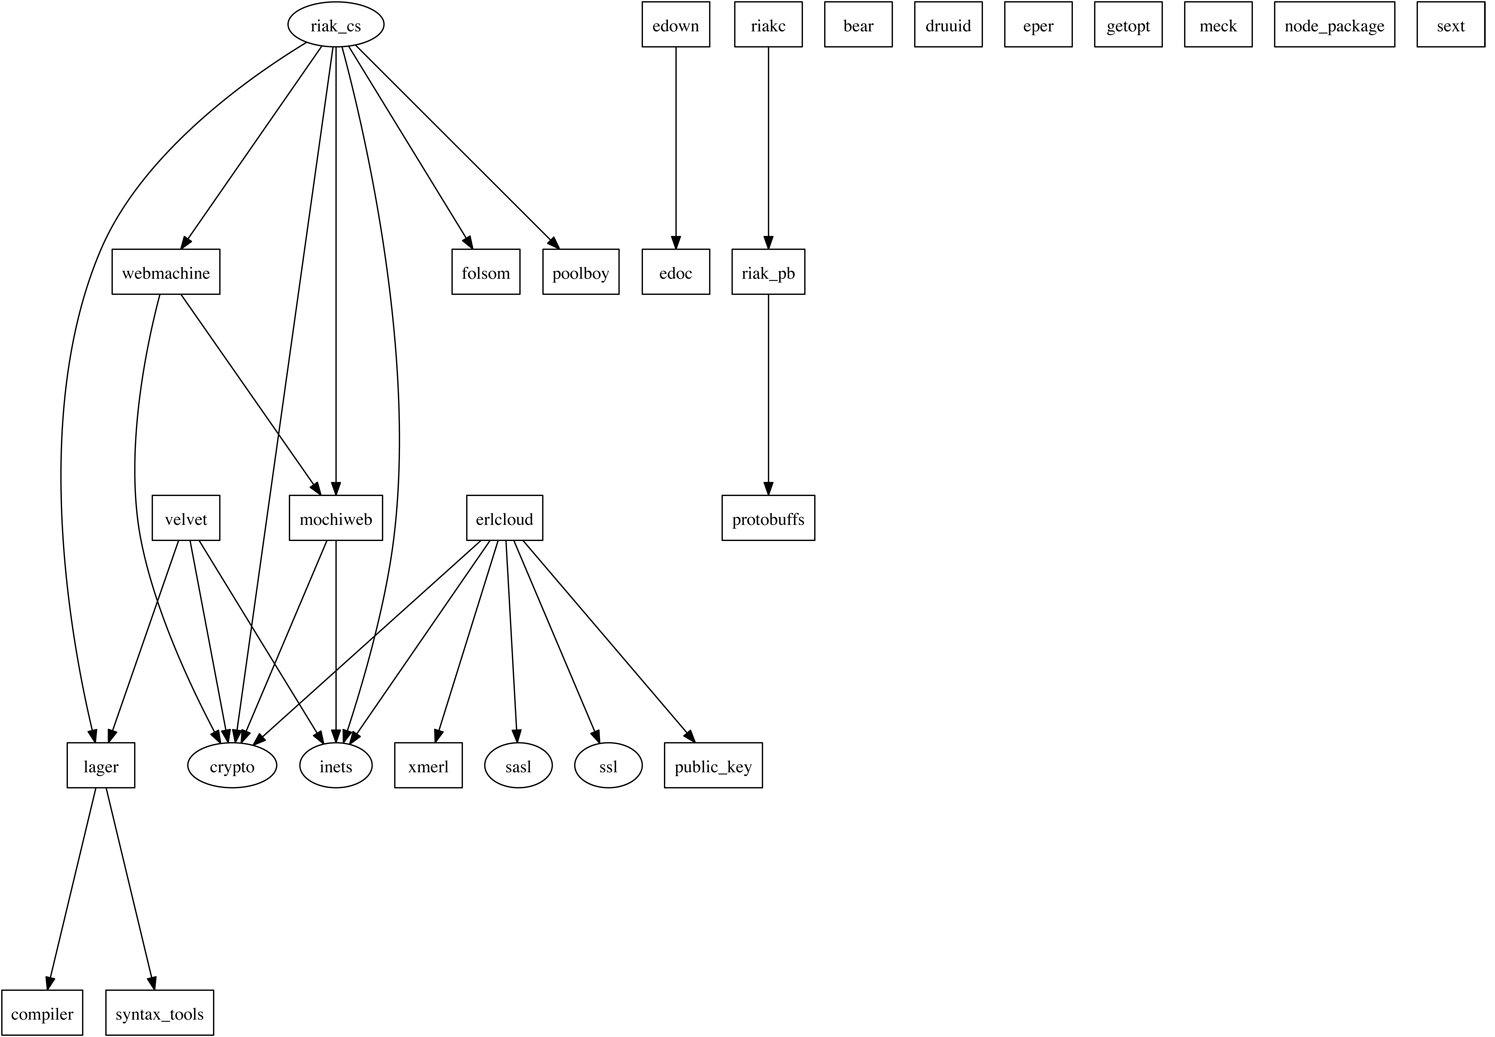
\includegraphics{app-deps-riak-cs.pdf}%
%  \caption{Dependency graph of riak\_cs, Basho's open source cloud library. The graph ignores dependencies on common applications like kernel and stdlib. Ovals are applications, rectangles are library applications.}%
  \caption{Граф зависимостей riak\_cs, облачной библиотеки с открытым исходным кодом, написанной компанией Basho. Граф игнорирует зависимости от общих приложений, таких как kernel и stdlib. Овалами показаны приложения, прямоугольниками --- библиотечные приложения.}%
   \label{fig:app-deps}
\end{figure}

%Using such a hierarchy and looking at each application's short description might be helpful to draw a rough, general map of where everything is located. To generate a similar diagram, find \app{recon}'s script directory and call \command{escript script/app\_deps.erl}\footnote{This script depends on graphviz}. Similar hierarchies can be found using the \module{observer}\footnote{\href{http://www.erlang.org/doc/apps/observer/observer\_ug.html}{http://www.erlang.org/doc/apps/observer/observer\_ug.html}} application, but for individual supervision trees. Put together, you may get an easy way to find out what does what in the code base.
Используя такую иерархию и глядя на короткое описание каждого из приложений, может оказаться полезным нарисовать приблизительную грубую карту где что находится. Для создания подобной диаграммы найдите в приложении \app{recon} директорию сценариев \filename{script/} и вызовите \command{escript script/app\_deps.erl}\footnote{Этот скрипт требует наличия у вас в системе программы graphviz}. Подобные иерархии можно найти используя \module{observer}\footnote{\href{http://www.erlang.org/doc/apps/observer/observer\_ug.html}{http://www.erlang.org/doc/apps/observer/observer\_ug.html}}, но для отдельных деревьев наблюдения. Если сложить это вместе, у вас может получиться удобный способ быстро нарисовать и разобраться, что происходит в незнакомом коде.


\FloatBarrier

\section{Ныряем в OTP-релизы}
\label{sec:dive-otp-releases}

%OTP releases are not a lot harder to understand than most OTP applications you'll encounter in the wild. A release is a set of OTP applications packaged in a production-ready manner so it boots and shuts down without needing to manually call \function{application:start/2} for any app. Of course there's a bit more to releases than that, but generally, the same discovery process used for individual OTP applications will be applicable here.
ОТР-релизы не сильно сложнее для понимания, чем обычные ОТР-приложения, которые могут вам встретиться в дикой природе. Релиз --- это набор ОТР-приложений, упакованных для доставки на производственные (\emph{production}) сервера так, что они запускаются и завершают работу без ручного вызова \function{application:start/2} в любом нужном вам приложении. Конечно есть и другие подробности касательно релизов, но обычно применяется тот же процесс исследования, как и для обычных приложений ОТР.

%You'll usually have a file similar to the configuration files used by \module{systools} or \module{reltool}, which will state all applications part of the release and a few\footnote{A lot} options regarding their packaging. To understand them, I recommend \href{http://learnyousomeerlang.com/release-is-the-word}{reading existing documentation on them}. If you're lucky, the project may be using \app{relx}\footnote{\href{https://github.com/erlware/relx/wiki}{https://github.com/erlware/relx/wiki}}, an easier tool that was officially released in early 2014.
Обычно у вас будет файл, похожий на файлы конфигурации, которыми пользуется  \module{systools} или \module{reltool}, который содержит перечень всех приложений, включённых в релиз и несколько\footnote{На самом деле множество.} параметров касательно способа их упаковки. Для лучшего их понимания я рекомендую обратиться к  \href{http://learnyousomeerlang.com/release-is-the-word}{чтению существующей документации и книгам}. Если вам повезло, проект мог быть собран с помощью \app{relx}\footnote{\href{https://github.com/erlware/relx/wiki}{https://github.com/erlware/relx/wiki}}, более удобного инструмента, который был официально выпущен в начале 2014.


\section{Упражнения}

\subsection*{\ReviewTitle{}}

\begin{enumerate}
%	\item How do you know if a code base is an application? A release?
	\item Как вы можете узнать, что данный код является приложением? Релизом?
%	\item What differentiates an application from a library application?
	\item Что отличает обычное приложение от библиотечного?
%	\item What can be said of processes under a \term{one\_for\_all} scheme for supervision?
	\item Что можно сказать о процессах, которые запускаются под наблюдателем по схеме \term{one\_for\_all}?
%	\item Why would someone use a \module{gen\_fsm} behaviour over a \module{gen\_server}?
	\item Почему кто-то может решить использовать поведение \module{gen\_fsm} вместо \module{gen\_server}?
\end{enumerate}

\subsection*{\HandsOnTitle{}}

%Download the code at \href{https://github.com/ferd/recon\_demo}{https://github.com/ferd/recon\_demo}. This will be used as a test bed for exercises throughout the book. Given you are not familiar with the code base yet, let's see if you can use the tips and tricks mentioned in this chapter to get an understanding of it.
Скачайте код отсюда: \href{https://github.com/ferd/recon\_demo}{https://github.com/ferd/recon\_demo}. Этот проект будет использоваться как основа для упражнений по всей книге. Подразумевается, что вы пока не знакомы с этим кодом, давайте посмотрим, как вы воспользуетесь знаниями, полученными в текущей главе и разберётесь что к чему.

\begin{enumerate}
%	\item Is this application meant to be used as a library? A standalone system?
	\item Задумано ли это приложение как библиотека или как отдельно работающая система?
%	\item What does it do?
	\item Что оно делает?
%	\item Does it have any dependencies? What are they?
	\item Есть ли у него зависимости? Какие?
%	\item The app's \filename{README} mentions being non-deterministic. Can you prove if this is true? How?
	\item Файл \filename{README} упоминает что-то о недетерминированности. Можете ли вы найти доказательства, что это правда? Как?
%	\item Can you express the dependency chain of applications in there? Generate a diagram of them?
	\item Можно ли здесь выразить цепочку зависимостей приложений? Создать диаграмму?
%	\item Can you add more processes to the main application than those described in the \filename{README}? 
	\item Можно ли добавить новые процессы к главному приложению кроме тех, что были описаны в файле \filename{README}?
\end{enumerate}
%%%
%%%
%%%

%%% Cognitive
%%
%% Knowledge: recall facts, terms, basic concepts
%% 
%% - How do you know if a code base is an application? A release?
%% - Where can you find what an application does?
%% - What differentiates an application from a library application?
%%
%% Comprehension: organizing, comparing, translating, interpreting, giving descriptions, and stating the main ideas
%%
%% - What can be said of processes under a one_for_all scheme for supervision?
%% - Why would someone use a gen_fsm process over a gen_server?
%%
%% Application: Solve problems in new situations by applying acquired knowledge, facts, techniques and rules in a different way
%%
%% Using the code at: https://github.com/ferd/recon_demo
%% - Is this application meant to be used as a library? A standalone system?
%% - What does it do?
%% - Does it have any dependencies? What are they?
%%
%% Analysis: break down info, make inferences, find evidence
%% - The app's readme mentions being non-deterministic. Can you prove if this is true? How?
%% - Can you express the dependency chain of applications in there? Generate a diagram of them?
%%
%% Synthesis: Compile information together in a different way by combining elements in a new pattern or proposing alternative solutions
%%
%% - Can you add more processes to the application? DO IT!
%%
%% Evaluation: Present and defend opinions by making judgments about information
%%
%% - Do you think the method you've chosen to add applications would work well operationally to be done live? If not, is this due to your choice or the application structure? 
%%

%%%
%%%
%%%

\chapter{Построение проектов с открытым исходным кодом на Erlang}
\label{chap:building-open-source-erlang-software}

%Most Erlang books tend to explain how to build Erlang/OTP applications, but few of them go very much in depth about how to integrate with the Erlang community doing Open Source work. Some of them even avoid the topic on purpose. This chapter dedicates itself to doing a quick tour of the state of affairs in Erlang.
Большинство книг по Erlang стараются объяснить, как построить приложения на Erlang/OTP, но совсем немногие углубляются в вопросы взаимодействия с сообществом, которое работает над приложениями с открытым исходным кодом (\emph{open source}). Некоторые даже специально избегают эту тему. Эта глава посвящена небольшой экскурсии по состоянию отношений между людьми и программами в Erlang.

%OTP applications are the vast majority of the open source code people will encounter. In fact, many people who would need to build an OTP release would do so as one umbrella OTP application. 
OTP-приложения являются подавляющим большинством исходных кодов, которые вы можете встретить. На самом деле многие люди, кому нужно собрать OTP-релиз, делают это в виде ещё одного приложения-зонтика, под которым размещаются все остальные части проекта.

%If what you're writing is a stand-alone piece of code that could be used by someone building a product, it's likely an OTP application. If what you're building is a product that stands on its own and should be deployed by users as-is (or with a little configuration), what you should be building is an OTP release.\footnote{The details of how to build an OTP application or release is left up to the Erlang introduction book you have at hand.}
Если то, что вы пишете, является отдельным набором файлов и кода, которые могут пригодиться кому-то ещё при построении их продукта, то вероятнее всего это будет оформлено, как приложение OTP.

%The main build tools supported are \app{rebar} and \app{erlang.mk}. The former is a portable Erlang script that will be used to wrap around a lot of standard functionality and add its own, while the latter is a very fancy makefile that does a bit less, but tends to be faster when it comes to compiling. In this chapter, I'll mostly focus on using \app{rebar} to build things, given it's the ad-hoc standard, is well-established, and \app{erlang.mk} applications tend to also be supported by \app{rebar} as dependencies.
Основные инструменты для сборки, которые получают поддержку авторов и сообщества --- это \app{rebar} и \app{erlang.mk}. Первое --- это портативный самодостаточный скрипт на языке Erlang, который является интерфейсом к ряду стандартных функций и добавляет некоторые свои, тогда как второе --- хитро закрученный стандартный сборочный файл (\emph{Makefile}), который делает немного меньше, но обычно выполняет компиляцию быстрее. В этой главе я в основном сосредоточусь на сборке с помощью \app{rebar}, поскольку он принят почти всеми, как стандарт, хорошо известен, а приложения, использующие \app{erlang.mk}, обычно поддерживаются при сборке с помощью \app{rebar} в качестве зависимостей.


\section{Структура проекта}
\label{sec:project-structure}

%The structures of OTP applications and of OTP releases are different. An OTP application can be expected to have one top-level supervisor (if any) and possibly a bunch of dependencies that sit below it. An OTP release will usually be composed of multiple OTP applications, which may or may not depend on each other. This will lead to two major ways to lay out applications.
Структуры приложений и релизов OTP отличаются. Ожидается, что OTP-приложение имеет один наблюдатель верхнего уровня (или ни одного) и, возможно, ряд зависимостей, которые находятся под ним. OTP-релиз обычно состоит из ряда ОТР-приложений, которые могут зависеть (или не зависеть) друг от друга. Это является причиной существования двух очень разных структур директорий.

\subsection{OTP-приложения}
\label{subsec:building-otp-applications}

%For OTP applications, the proper structure is pretty much the same as what was explained in \ref{sec:dive-otp-applications}:
Для ОТР-приложений правильной структурой является точно такая же, как мы рассмотрели ранее в секции \ref{sec:dive-otp-applications}:

\begin{VerbatimText}
doc/
deps/
ebin/
src/
test/
LICENSE.txt
README.md
rebar.config
\end{VerbatimText}

%What's new in this one is the \filename{deps/} directory, which is fairly useful to have, but that will be generated automatically by \app{rebar}\footnote{A lot of people package \app{rebar} directly in their application. This was initially done to help people who had never used rebar before use libraries and projects in a boostrapped manner. Feel free to install rebar globally on your system, or keep a local copy if you require a specific version to build your system.} if necessary. That's because there is no canonical package management in Erlang. People instead adopted \app{rebar}, which fetches dependencies locally, on a per-project basis. This is fine and removes a truckload of conflicts, but means that each project you have may have to download its own set of dependencies.
Какие появились отличия --- это директория \filename{deps/}, которую полезно иметь и она будет создана автоматически при работе с \app{rebar}\footnote{Многие люди пакуют \app{rebar} прямо в свои приложения. Изначально это помогало другим людям, которые никогда ранее им не пользовались, начать немедленно им пользоваться. На ваш вкус можно установить rebar глобально в вашей системе, или хранить локальную копию, если вам требуется особенная его версия.} по мере необходимости. Это происходит потому, что Erlang не имеет стандартного управления пакетами зависимостей. Вместо этого люди решили использовать \app{rebar}, который скачивает зависимости локально для каждого проекта свои. Это приемлемое решение и убирает массу проблем с конфликтами, но означает, что каждому проекту придётся скачивать свой набор зависимостей.

%This is accomplished with \app{rebar} by adding a few config lines to \filename{rebar.config}:
Зависимости для \app{rebar} задаются с помощью добавления строк в специальный файл \filename{rebar.config}, которого ваш проект может не иметь --- тогда создайте его сами:

\begin{VerbatimText}
{deps,
 [{application_name, "1.0.*",
   {git, "git://github.com/user/myapp.git", {branch,"master"}}},
  {application_name, "2.0.1",
   {git, "git://github.com/user/hisapp.git", {tag,"2.0.1"}}},
  {application_name, "", 
   {git, "https://bitbucket.org/user/herapp.git",  "7cd0aef4cd65"}},
  {application_name, "my regex",
   {hg, "https://bitbucket.org/user/theirapp.hg" {branch, "stable"}}}]}.
\end{VerbatimText}

%Applications are fetched directly from a \app{git} (or \app{hg}, or \app{svn}) source, recursively. They can then be compiled, and specific compile options can be added with the \expression{\{erl\_opts, List\}.} option in the config file\footnote{More details by calling \command{rebar help compile}}.
Приложения и их зависимости скачиваются рекурсивно с помощью стандартных утилит \app{git} (или \app{hg}, или \app{svn}) с указанных серверов. Затем они готовы к сборке и вы можете добавить особые параметры компиляции с помощью строки \expression{\{erl\_opts, СписокПараметров\}.} в файле конфигурации\footnote{Можно узнать подробнее, если выполнить \command{rebar help compile}}.

%Within these directories, you can do your regular development of an OTP application. To compile them, call \command{rebar get-deps compile}, which will download all dependencies, and then build them and your app at once.
В пределах этих директорий вы можете выполнять обычную разработку вашего ОТР-приложения. Для компиляции вызовите команду \command{rebar get-deps compile}, которая докачает недостающие зависимости и затем соберёт всё вместе с вашим приложением.

%When making your application public to the world, distribute it \emph{without} the dependencies. It's quite possible that other developers' applications depend on the same applications yours do, and it's no use shipping them all multiple times. The build system in place (in this case, \app{rebar}) should be able to figure out duplicated entries and fetch everything necessary only once.
Когда вы публикуете ваше приложение для всех желающих, то зависимости \emph{не включаются} в архив. Вполне возможна ситуация, когда приложения другого разработчика зависят от тех же приложений, что и ваше, и нет смысла поставлять ему наши копии зависимостей. Система сборки на компьютере другого разработчика (в нашем случае, \app{rebar}) сможет разобраться, какие зависимости нужны и докачает недостающие.

%% erlang.mk downloads relx for releases, and runs it iff there's a relx file there

\subsection{Строим OTP-релизы}
\label{subsec:building-otp-releases}

%For releases, the structure should be a bit different\footnote{I say \emph{should} because many Erlang developers put their final system under a single top-level application (in \filename{src}) and a bunch of follower ones as dependencies (in \filename{deps}), which is less than ideal for distribution purposes and conflicts with assumptions on directory structures made by OTP. People who do that tend to build from source on the production servers and run custom commands to boot their applications.}. Releases are collections of applications, and their structures should reflect that.
Для релизов структура должна немного отличаться\footnote{Я пишу \emph{должна} потому что многие Erlang-разработчики размещают свою готовую программу в единственном приложении на верхнем уровне проекта (в папке \filename{src/}) и ряд вспомогательных приложений оформляются, как зависимости (в папке \filename{deps/}), что не совсем идеально для нужд распространения программы и конфликтует с рекомендуемой стандартом ОТР структурой директорий. Люди, которые так делают, обычно собирают код из исходников при установке на производственные сервера и выполняют особые самодельные команды для их запуска.}. Релизы --- это наборы приложений, и их структура должна отражать этот факт.

%Instead of having a top-level app, applications should be nested one level deeper and divided into two categories: apps and deps. The apps directory contains your applications' source code (say, internal business code), and the deps directory contains independently managed dependency applications.
Вместо того, чтобы делать одно приложение верхнего уровня, следует разместить все приложения на один уровень глубже и разделить на две категории: собственно приложения (\emph{apps}) и зависимости (\emph{deps}). Директория \filename{apps/} содержит исходный код вашего приложения (скажем, ваша бизнес-логика), а директория \filename{deps/} содержит ваши зависимости, управляемые другими авторами или командами.

\begin{VerbatimRaw}
apps/
doc/
deps/
LICENSE.txt
README.md
rebar.config
\end{VerbatimRaw}

%This structure lends itself to generating releases. Tools such as Systool and Reltool have been covered before\footnote{\href{http://learnyousomeerlang.com/release-is-the-word}{http://learnyousomeerlang.com/release-is-the-word}}, and can allow the user plenty of power. An easier tool that recently appeared is \app{relx}\footnote{\href{https://github.com/erlware/relx/wiki}{https://github.com/erlware/relx/wiki}}.
Эта структура годится для генерации релизов. Инструменты, такие как Systool и Reltool были описаны в других публикациях\footnote{\href{http://learnyousomeerlang.com/release-is-the-word}{http://learnyousomeerlang.com/release-is-the-word}}, и могут дать пользователю большую власть. Более лёгкий инструмент, который появился совсем недавно --- это \app{relx}\footnote{\href{https://github.com/erlware/relx/wiki}{https://github.com/erlware/relx/wiki}}.

%A  \app{relx} configuration file for the directory structure above would look like:
Файл конфигурации для \app{relx}, описывающий структуру директорий, показанную выше, будет выглядеть так:

\begin{VerbatimText}
{paths, ["apps", "deps"]}.
{include_erts, false}. % релиз будет использовать установленный в системе Erlang
{default_release, demo, "1.0.0"}.

{release, {demo, "1.0.0"},
    [members,
     feedstore,
     ...
     recon]}.
\end{VerbatimText}

%Calling \command{./relx} (if the executable is in the current directory) will build a release, to be found in the \filename{\_rel/} directory. If you really like using \app{rebar}, you can build a release as part of the project's compilation by using a rebar hook in \filename{rebar.config}:
Вызов команды \command{./relx} (если исполняемый файл relx находится в текущей директории) начнёт сборку релиза, который будет помещён в директорию \filename{\_rel/}. Если вам нравится пользоваться программой \app{rebar}, то вы можете построить релиз в процессе компиляции проекта используя такую строчку в \filename{rebar.config}:

\begin{VerbatimText}
{post_hooks,[{compile, "./relx"}]}.
\end{VerbatimText}

%And every time \command{rebar compile} will be called, the release will be generated.
Тогда каждый раз, когда вы вызовете команду \command{rebar compile}, будет создаваться релиз.

\section{Наблюдатели и семантика start\_link}
\label{sec:supervisors-and-start-link-semantics}

%In complex production systems, most faults and errors are transient, and retrying an operation is a good way to do things — Jim Gray's paper\footnote{\href{http://mononcqc.tumblr.com/post/35165909365/why-do-computers-stop}{http://mononcqc.tumblr.com/post/35165909365/why-do-computers-stop}} quotes \emph{Mean Times Between Failures} (MTBF) of systems handling transient bugs being better by a factor of 4 when doing this. Still, supervisors aren't just about restarting.
В сложной производственной (\emph{production}) системе многие сбои и ошибки являются временными, и повторная попытка выполнить операцию --- это хороший подход к ведению дел, согласно работе Джима Грэй \footnote{\href{http://mononcqc.tumblr.com/post/35165909365/why-do-computers-stop}{http://mononcqc.tumblr.com/post/35165909365/why-do-computers-stop}}, которая цитирует, что \emph{среднее время наработки до отказа} (\emph{Mean Times Between Failures или сокращённо MTBF}) систем, которые обрабатывают такие временные ошибки, улучшается в 4 раза. И всё же тема наблюдателей затрагивает больше, чем просто перезапуски.

%One very important part of Erlang supervisors and their supervision trees is that \emph{their start phases are synchronous}. Each OTP process has the potential to prevent its siblings and cousins from booting. If the process dies, it's retried again, and again, until it works, or fails too often.
Одним из важных фактов о наблюдателях в Erlang и их деревьях наблюдения является то, что \emph{фазы их запуска синхронны}. Каждый процесс в OTP имеет возможность заблокировать запуск своих дочерних и сестринских процессов. Если процесс завершается аварийно (умирает), то попытка повторяется снова и снова, пока он не запустится успешно или наблюдатель не сочтёт, что процесс падает слишком часто.

%That's where people make a very common mistake. There isn't a backoff or cooldown period before a supervisor restarts a crashed child. When a network-based application tries to set up a connection during its initialization phase and the remote service is down, the application fails to boot after too many fruitless restarts. Then the system may shut down.
Здесь люди часто делают одну общую ошибку. Нет никакой паузы перед тем, как наблюдатель перезапускает упавший дочерний процесс. Когда сетевое приложение пытается установить подключение во время фазы своей инициализации в то время, как удалённый сервис не работает, приложение не может загрузиться после ряда безуспешных перезапусков. Затем система останавливается целиком.

%Many Erlang developers end up arguing in favor of a supervisor that has a cooldown period. I strongly oppose the sentiment for one simple reason: \emph{it's all about the guarantees}.
Много Erlang-разработчиков скатываются в споры о создании наблюдателя, который бы имел период ожидания между перезапусками. Я выступаю против этой идеи по одной простой причине: \emph{дело в том, какие вы получаете гарантии}.

\subsection{Всё дело в гарантии}
\label{subsec:start-link-guarantees}

%Restarting a process is about bringing it back to a stable, known state. From there, things can be retried. When the initialization isn't stable, supervision is worth very little. An initialized process should be stable no matter what happens. That way, when its siblings and cousins get started later on, they can be booted fully knowing that the rest of the system that came up before them is healthy.
Перезапуск процесса --- это перевод его в стабильное и заранее известное состояние. С этого момента можно повторно выполнять какие-то неудачные операции. Если инициализация нестабильна, то наблюдение за процессом не стоит и гроша. Инициализированный начисто процесс должен быть стабильным что бы ни произошло. Таким образом, когда дочерние и сестринские процессы перезапустятся в будущем, они будут уверены в том, что остальная система, запущенная до них, в хорошем состоянии и исправна.

%If you don't provide that stable state, or if you were to start the entire system asynchronously, you would get very little benefit from this structure that a \expression{try ... catch} in a loop wouldn't provide.
Если вы не обеспечите такое стабильное состояние, или если вы запускаете всю систему асинхронно, то такая структура даст вам мало преимуществ по сравнению с запуском \expression{try} ... \expression{catch} в цикле.

%Supervised processes \emph{provide guarantees} in their initialization phase, \emph{not a best effort}. This means that when you're writing a client for a database or service, you shouldn't need a connection to be established as part of the initialization phase unless you're ready to say it will always be available no matter what happens.
Процессы под наблюдением \emph{обеспечивают гарантии} в фазе их инициализации, в отличие от \emph{попыток сделать всё возможное}. Это означает, что когда вы пишете клиент для базы данных или сервис, вам не потребуется проверять наличие подключения в ходе фазы инициализации, если вы можете утверждать, что оно всегда будет доступно вне зависимости от ситуации.

%You could force a connection during initialization if you know the database is on the same host and should be booted before your Erlang system, for example. Then a restart should work. In case of something incomprehensible and unexpected that breaks these guarantees, the node will end up crashing, which is desirable: a pre-condition to starting your system hasn't been met. It's a system-wide assertion that failed.
Например вы могли бы принудительно выполнить подключение во время инициализации, если вы знаете, что база данных находится на одном с вами сервере и должна запуститься до старта вашей Erlang-системы. Тогда перезапуск сработал бы. В случае, если случится нечто непонятное и неожиданное, нарушающее эти гарантии, то ваш узел завершит работу аварийно, что вполне нам подходит: предварительное условие для запуска системы не было выполнено. Обязательная для старта системы тестовая проверка не прошла.

%If, on the other hand, your database is on a remote host, you should expect the connection to fail. It's just a reality of distributed systems that things go down.\footnote{Or latency shoots up enough that it is impossible to tell the difference from failure.} In this case, the only guarantee you can make in the client process is that your client will be able to handle requests, but not that it will communicate to the database. It could return \expression{\{error, not\_connected\}} on all calls during a net split, for example.
Если же, с другой стороны, ваша база данных находится на удалённом сервере, то следует быть готовыми к тому, что подключение завершится неудачей. Это повседневная реальность распределённых систем --- их части постоянно отказывают\footnote{Или сетевая задержка увеличивается настолько, что становится трудно отличить ситуацию от полного отказа.}. В таком случае единственной гарантией, которую вы можете обеспечить в клиенстком процессе будет то, что ваш клиент сможет обработать запросы, но не подключиться к базе данных. Например, он мог бы возвращать \expression{\{error,} \expression{not\_connected\}} на все вызовы во время разделения сети.

%The reconnection to the database can then be done using whatever cooldown or backoff strategy you believe is optimal, without impacting the stability of the system. It can be attempted in the initialization phase as an optimization, but the process should be able to reconnect later on if anything ever disconnects.
Повторное подключение к базе данных затем может произойти с любой удобной вам частотой или задержкой, не влияя на стабильность работы системы. Попытка также может быть выполненя в фазе инициализации, в качестве оптимизации, но процесс должен уметь повторно подключиться позже в случае отказа или отключения.

%If you expect failure to happen on an external service, do not make its presence a guarantee of your system. We're dealing with the real world here, and failure of external dependencies is always an option. 
Если вы ожидаете, что внешний сервис откажет, не делайте его наличие обязательной гарантией для вашей системы. Мы здесь работаем с реальным миром, и отказ внешних зависимостей может произойти в любой момент.


\subsection{Побочные эффекты}
\label{subsec:start-link-side-effects}

%Of course, the libraries and processes that call such a client will then error out if they don't expect to work without a database. That's an entirely different issue in a different problem space, one that depends on your business rules and what you can or can't do to a client, but one that is possible to work around. For example, consider a client for a service that stores operational metrics — the code that calls that client could very well ignore the errors without adverse effects to the system as a whole. 
Само собой, библиотеки и процессы, которые используют такой клиент, могут вылететь с ошибкой, если они не ожидают неожиданно оказаться без базы данных. Эта проблема совсем иная и лежит в другой плоскости, которая зависит от правил вашей бизнес-логики и того, что вы можете или не можете делать с клиентом, но проблема вполне решаемая. Например, представьте себе клиент некоторого сервиса, хранящий операционные метрики --- код, который вызывает этого клиента, может игнорировать ошибки и они не окажут ощутимого влияния на работу системы в целом.

%The difference in both initialization and supervision approaches is that the client's callers make the decision about how much failure they can tolerate, not the client itself. That's a very important distinction when it comes to designing fault-tolerant systems. Yes, supervisors are about restarts, but they should be about restarts to a stable known state.
Разница в подходах к инициализации и наблюдению за процессами в том, что не наш клиент, а вызывающие его процессы принимают решение о том, насколько они готовы терпеть сбои и ошибки. Это очень важное различие, когда дело касается проектирования устойчивых к сбоям систем. Да, наблюдатели только и делают, что занимаются перезапусками, но суть в том, что перезапуски должны приводить к стабильному и известному заранее состоянию.


%\subsection{Example: Initializing without guaranteeing connections}
\subsection{Пример: Инициализация без гарантии подключения}
\label{subsec:start-link-initializing-without-guaranteeing-connections}

%The following code attempts to guarantee a connection as part of the process' state:
Следующий код пытается гарантировать наличие живого соединения при запуске процесса:

\begin{VerbatimText}
init(Args) ->
    Opts = parse_args(Args),
    {ok, Port} = connect(Opts),
    {ok, #state{sock=Port, opts=Opts}}.

[...]

handle_info(reconnect, S = #state{sock=undefined, opts=Opts}) ->
    %% попытаемся подключиться в цикле
    case connect(Opts) of
        {ok, New} -> {noreply, S#state{sock=New}};
         _ -> self() ! reconnect, {noreply, S}
    end;
\end{VerbatimText}

%Instead, consider rewriting it as:
Вместо этого попробуйте переписать его так:

\begin{VerbatimText}
init(Args) ->
    Opts = parse_args(Args),
    %% вы всё равно можете попытаться подключиться прямо здесь, чтобы по 
    %% возможности улучшить доступность, но будьте готовы, что подключение 
    %% не удастся
    self() ! reconnect,
    {ok, #state{sock=undefined, opts=Opts}}.

[...]

handle_info(reconnect, S = #state{sock=undefined, opts=Opts}) ->
    %% попытаемся подключиться в цикле
    case connect(Opts) of
        {ok, New} -> {noreply, S#state{sock=New}};
        _ -> self() ! reconnect, {noreply, S}
    end;
\end{VerbatimText}

%You now allow initializations with fewer guarantees: they went from \emph{the connection is available} to \emph{the connection manager is available}.
\sloppy{}
Теперь вы можете позволить инициализацию с меньшим количеством гарантий: раньше требовалась гарантия \emph{наличия подключения}, а сейчас требуется просто \emph{наличие менеджера подключений}.


\subsection{В двух словах}
\label{subsec:start-link-in-a-nutshell}

%Production systems I have worked with have been a mix of both approaches.
Производственные (\emph{production}) системы, с которыми мне довелось работать, использовали и тот и другой подход.

%Things like configuration files, access to the file system (say for logging purposes), local resources that can be depended on (opening UDP ports for logs), restoring a stable state from disk or network, and so on, are things I'll put into requirements of a supervisor and may decide to synchronously load no matter how long it takes (some applications may just end up having over 10 minute boot times in rare cases, but that's okay because we're possibly syncing gigabytes that we \emph{need} to work with as a base state if we don't want to serve incorrect information.)
Такие вещи, как файлы конфигурации, доступ к файловой системе (например, для потребностей ведения файлов журналов), локальные ресурсы, от которых могла бы зависеть система (открытие UDP-портов для ведения журналов), восстановление стабильного состояния из диска или по сети и так далее. Это те вещи, которые я помещаю в требования к наблюдателю и могу решить загрузить их синхронно независимо от того, сколько бы это ни потребовало времени (некоторые приложения иногда могут требовать более десяти минут для запуска, но это приемлемо, поскольку мы в этот момент перелопачиваем гигабайты, которые нам \emph{нужны} для работы в качестве базового состояния, если мы не хотим отдавать клиентам некорректные или неполные ответы).

%On the other hand, code that depends on non-local databases and external services will adopt partial startups with quicker supervision tree booting because if the failure is expected to happen often during regular operations, 
%then there's no difference between now and later. You have to handle it the same, and for these parts of the system, far less strict guarantees are often the better solution.
С другой стороны код, который зависит от удалённых баз данных и внешних сервисов, будет использовать запуск с частичными подключениями для ускорения запуска деревьев наблюдения, поскольку сбои ожидаются достаточно часто во время обычной работы, то и нет разницы в том, случится ли сбой при запуске или позже. Ваш подход к обработке этих ситуаций будет одинаковым, и для этих частей системы намного лучшим решением будет уменьшение гарантий.


%Application Strategies
\subsection{Стратегии приложений}
\label{subsec:start-link-application-strategies}

%No matter what, a sequence of failures is not a death sentence for the node. Once a system has been divided into various OTP applications, it becomes possible to choose which applications are vital or not to the node. Each OTP application can be started in 3 ways: temporary, transient, permanent, either by doing it manually in \expression{application:start(Name, Type)}, or in the config file for your release:
\sloppy{}
Вне зависимости от того, что произошло, ряд отказов не является смертельным приговором для узла. Как только система разделена на различные ОТР-приложения, становится возможным выбирать, какие из приложений являются жизненно-важными для узла. Каждое из приложений в ОТР может запускаться в трёх режимах: как временное (\emph{temporary}), преходящее или недолговечное (\emph{transient}) или постоянное (\emph{permanent}). Это делается либо вручную, выполняя команду \expression{application:start(Имя, Тип)}, либо из файла конфигурации вашего релиза:

\begin{itemize*}
%	\item \term{permanent}: if the app terminates, the entire system is taken down, excluding manual termination of the app with \function{application:stop/1}.
	\item Постоянное (\term{permanent}): если приложение завершит работу, то вся система останавливается, кроме тех случаев, когда приложение было остановлено вручную командой \function{application:stop/1}.
%	\item \term{transient}: if the app terminates for reason \term{normal}, that's ok. Any other reason for termination shuts down the entire system.
	\item Преходящее (\term{transient}): если приложение завершится по причине \term{normal}, то всё в порядке. Любая другая причина завершения работы останавливает всю систему.
%	\item \term{temporary}: the application is allowed to stop for any reason. It will be reported, but nothing bad will happen.
	\item Временное (\term{temporary}): приложению разрешено останавливаться нормально и аварийно, по любой причине. О ситуации будет доложено в журналы или на экран, но ничего плохого больше не произойдёт.
\end{itemize*}

%It is also possible to start an application as an \emph{included application}, which starts it under your own OTP supervisor with its own strategy to restart it.
Также возможно запустить приложение в качестве \emph{вложенного приложения} (\emph{included application}), что запустит его под наблюдателем ОТР со своей собственной стратегией перезапуска.


\section{Упражнения}

\subsection*{\ReviewTitle}

\begin{enumerate}
%	\item  Are Erlang supervision trees started depth-first? breadth-first? Synchronously or asynchronously?
	\item Запускаются ли деревья наблюдения в Erlang в глубину или в ширину? Синхронно или асинхронно?
%	\item What are the three application strategies? What do they do?
	\item Какие бывают три стратегии приложений? Что они делают?
%	\item What are the main differences between the directory structure of an app and a release?
	\item Какие главные различия между структурами директорий приложения и релиза?
%	\item When should you use a release?
	\item Когда следует использовать релиз?
%	\item Give two examples of the type of state that can go in a process' init function, and two examples of the type of state that shouldn't go in a process' init function
	\item Дайте два примера состояний, которые могут быть помещены в функцию инициализации процесса и два примера состояний, которые не следует туда помещать.
\end{enumerate}

\subsection*{\HandsOnTitle{}}

%Using the code at
Используйте код, который находится по адресу
\href{https://github.com/ferd/recon\_demo}{https://github.com/ferd/recon\_demo}:

\begin{enumerate}
%	\item Extract the main application hosted in the release to make it independent, and includable in other projects.
	\item Извлеките главное приложение, которое хранится в релизе, и сделайте его независимым с возможностью включения в другие проекты.
%	\item Host the application somewhere (Github, Bitbucket, local server), and build a release with that application as a dependency.
	\item Разместите приложение где-нибудь (Github, Bitbucket или ваш собственный сервер) и соберите релиз с этим приложением в качестве зависимости.
%	\item The main application's workers (\module{council\_member}) starts a server and connects to it in its \function{init/1} function. Can you make this connection happen outside of the init function's? Is there a benefit to doing so in this specific case?
	\item Рабочий процесс главного приложения (\module{council\_member}) запускает сервер и подключается к нему в своей функции \function{init/1}. Можно ли сделать это подключение за пределами функции init? Есть ли выгода от этого в данном конкретном случае?
\end{enumerate}

%%
%% Knowledge: recall facts, terms, basic concepts
%% 
%% - Does Erlang have package management? Where do dependencies live in a system?
%% - What are the commands to build an Erlang project using rebar?
%% - What tools are available to build releases?
%% - Are Erlang supervision trees started depth-first? breadth-first? Synchronously or asynchronously?
%% - What are the three application strategies?
%%
%% Comprehension: organizing, comparing, translating, interpreting, giving descriptions, and stating the main ideas
%%
%% - What are the main differences between the directory structure of an app? of a release?
%% - When should you use a release?
%%
%% Application: Solve problems in new situations by applying acquired knowledge, facts, techniques and rules in a different way
%%
%% Using the code at: https://github.com/ferd/recon_demo
%% - Extract the main application hosted in the release to make it independent, and includable in other projects
%% - Build a release with the app that was turned as a dependency
%%
%% Analysis: break down info, make inferences, find evidence
%% - Give two examples of the type of state that can go in a process' init function
%% - Give two examples of the type of state that should not go in a process' init function
%%
%% Synthesis: Compile information together in a different way by combining elements in a new pattern or proposing alternative solutions
%%
%% - Give example of applications you would design as temporary, transient, and permanent
%%
%% Evaluation: Present and defend opinions by making judgments about information
%%
%% - Do you think OTP supervisors should offer a back-off strategy on restart?
%% - What are the build tools you would choose for your app?
%%

%%%
%%%
%%%

%Planning for Overload
\chapter{В ожидании перегрузки}
\label{chap:overload}

%By far, the most common cause of failure I've encountered in real-world scenarios is due to the node running out of memory. Furthermore, it is usually related to message queues going out of bounds.\footnote{Figuring out that a message queue is the problem is explained in Chapter \ref{chap:crash-dumps}, specifically in Section \ref{sec:crash-full-mailboxes}} There are plenty of ways to deal with this, but knowing which one to use will require a decent understanding of the system you're working on.
Без сомнения одной из самых частых причин сбоев, которые мне встречались в ситуациях реального мира, это переполнение памяти на узлах. Более того, обычно это связано с очередями сообщений, которые растут бесконтрольно\footnote{Как разобраться, что именно очередь сообщений оказалась проблемой, объясняется в Главе \ref{chap:crash-dumps}, а именно в Секции \ref{sec:crash-full-mailboxes}}. Есть множество способов справиться с этой бедой, но выбор правильного решения потребует хорошего понимания системы, с которой вам довелось работать.

%To oversimplify things, most of the projects I end up working on can be visualized as a very large bathroom sink. User and data input are flowing from the faucet. The Erlang system itself is the sink and the pipes, and wherever the output goes (whether it's a database, an external API or service, and so on) is the sewer system.
Если говорить упрощённо, то большинство проектов, с которыми мне пришлось работать, могут быть изображены в виде кухонной раковины. Пользовательские и входящие данные вытекают из крана. Erlang-система является раковиной и трубами, а то, куда идёт вывод результатов (неважно, что это, база данных или внешний сервис) --- является канализацией.

\begin{figure}[h!]
  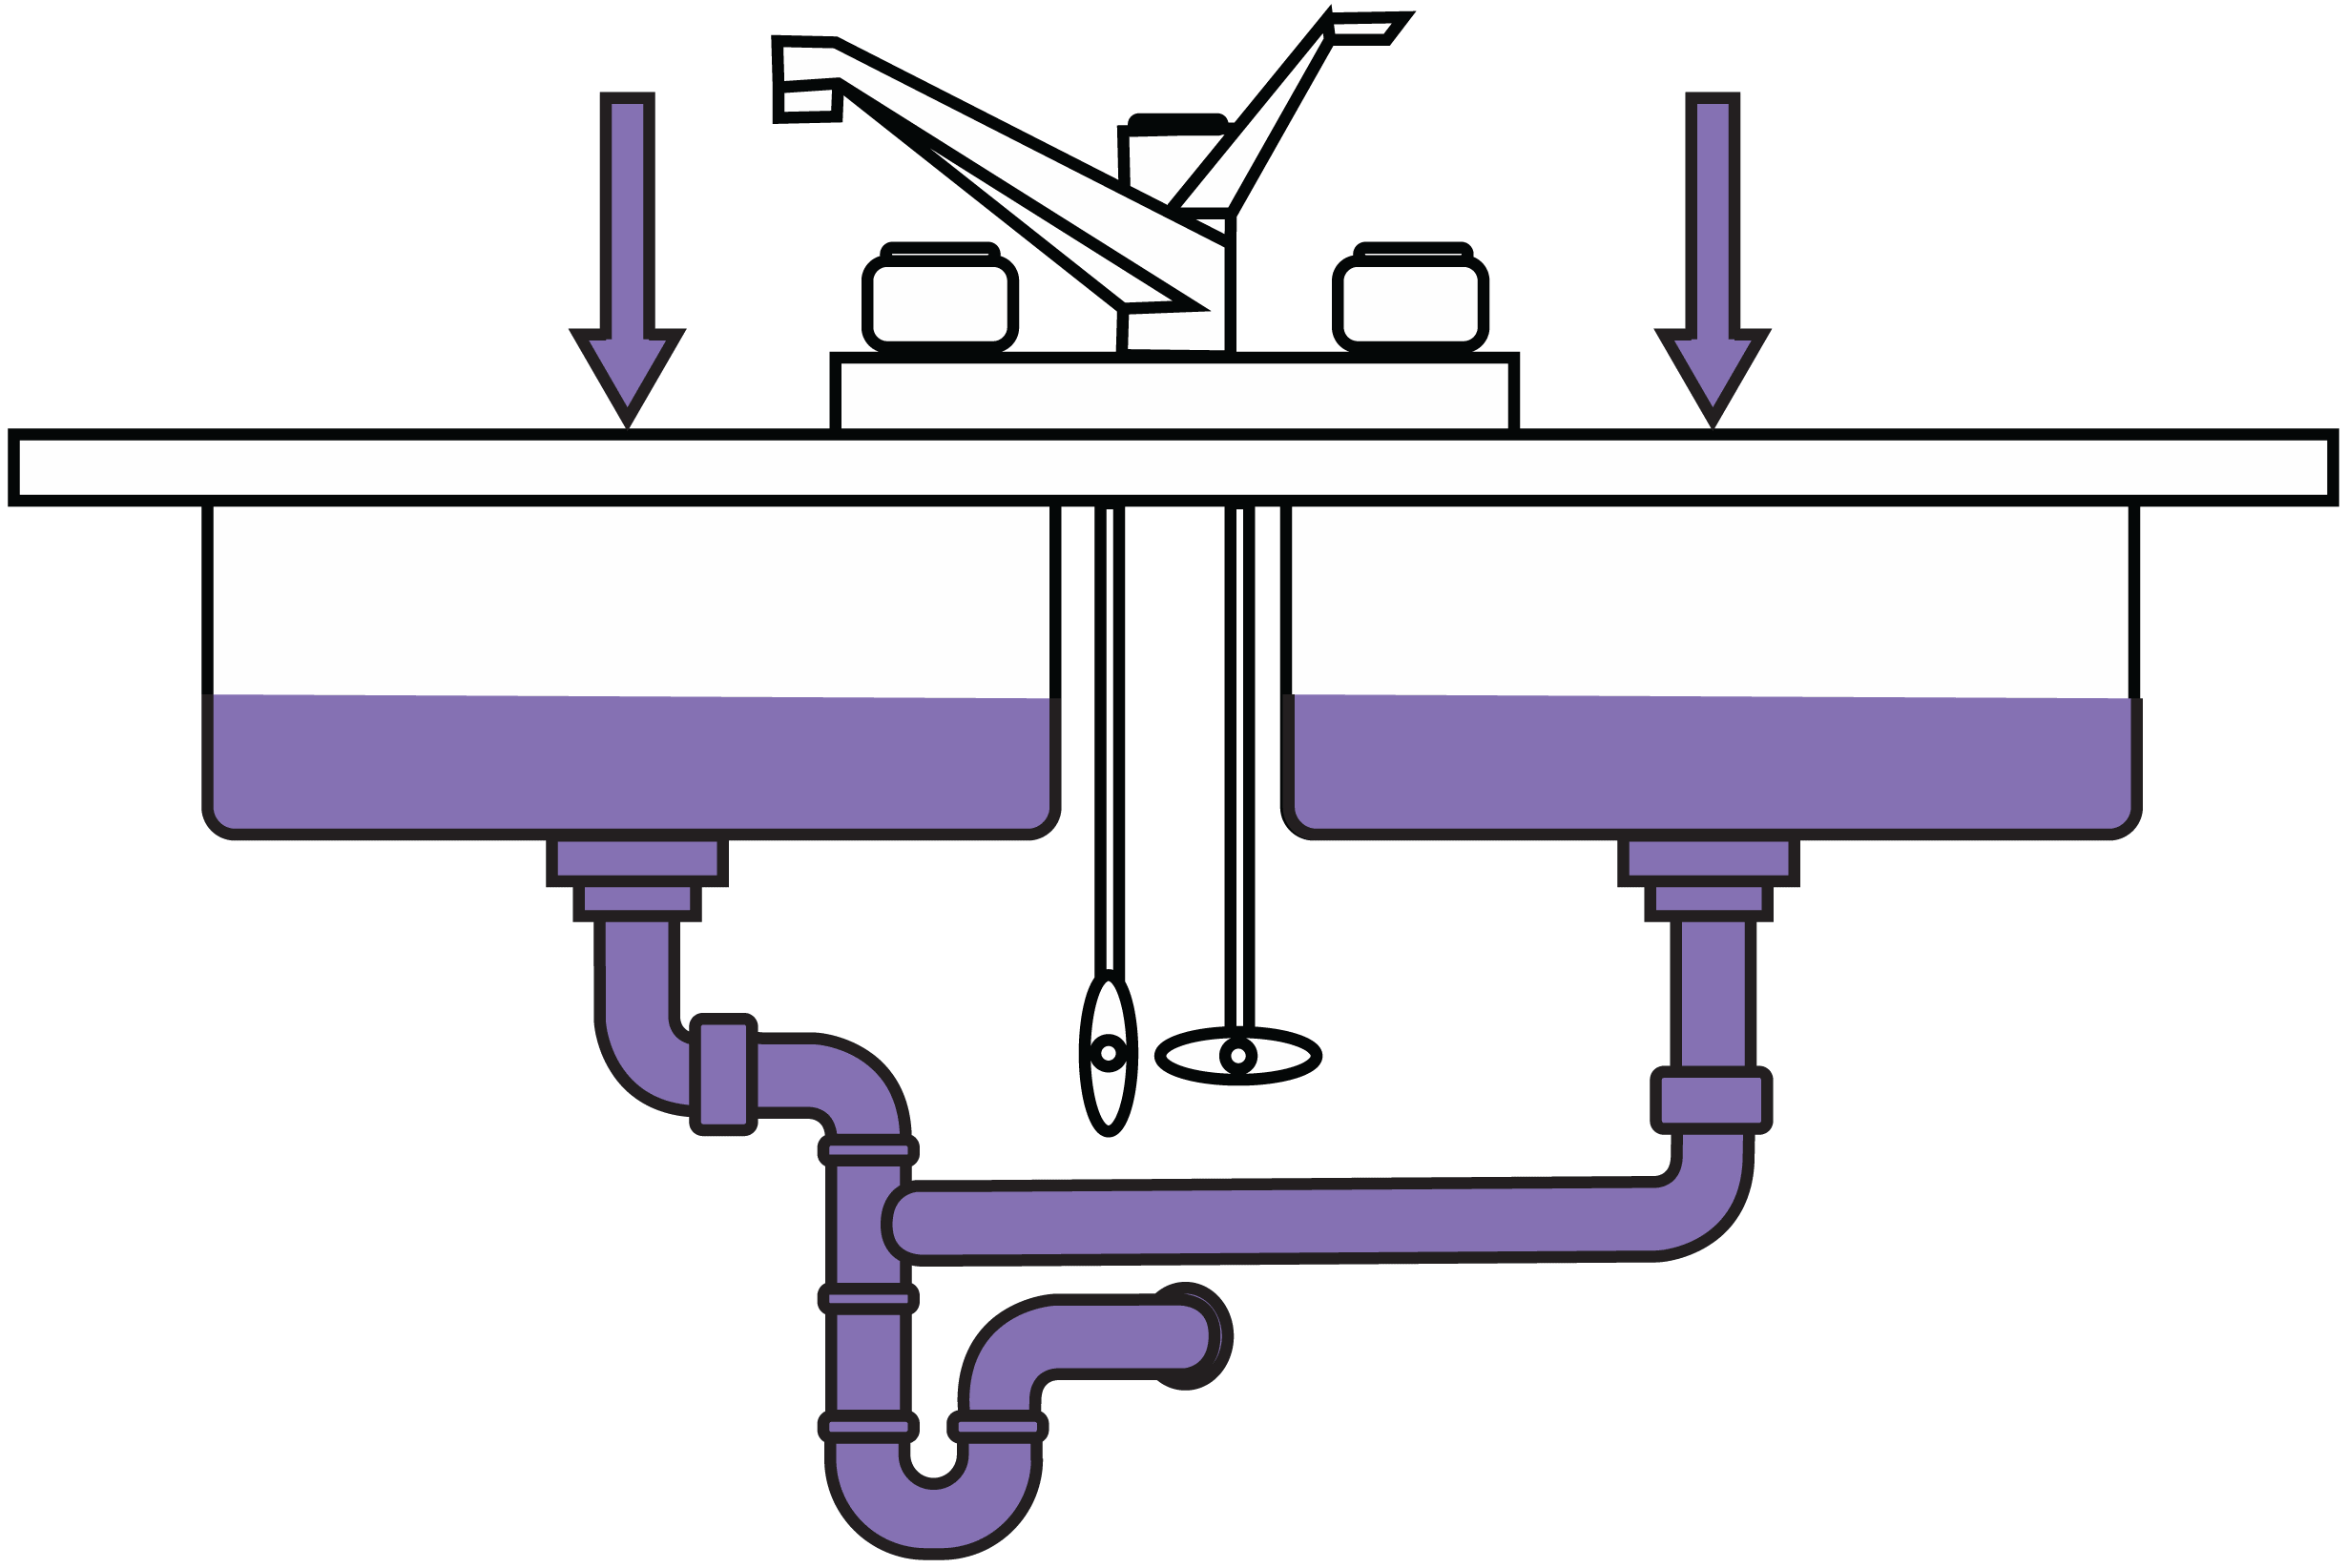
\includegraphics[max height=7cm]{sink.pdf}%
  \centering%
%  \caption{Your system is like a sink, and the true bottleneck, at the last drain, needs to be identified before you spend all your time and money making the sink and pipes bigger.}%
%\caption{Ваша система в виде раковины, и настоящее узкое место в последней трубе должно быть обнаружено до того, как вы потратите слишком много времени и денег увеличивая трубы и раковину.}
   \label{fig:tracing-venn}
\end{figure}

%When an Erlang node dies because of a queue overflowing, figuring out who to blame is crucial. Did someone put too much water in the sink? Are the sewer systems backing up? Did you just design too small a pipe?
Когда узел Erlang умирает по причине переполнения очереди, очень важно найти виновного. Вдруг налили слишком много воды? Справляется ли канализация? Не занизили ли вы размеры труб в проекте?

%Determining what queue blew up is not necessarily hard. This is information that can be found in a crash dump. Finding out why it blew up is trickier. Based on the role of the process or run-time inspection, it's possible to figure out whether causes include fast flooding, blocked processes that won't process messages fast enough, and so on.
Определить, какая из очередей взлетела на воздух будет нетрудно. Эту информацию можно обнаружить в файле дампа после смерти узла. А вот поиск причины, по которой это произошло --- более хитрая задача. Основываясь на роли процесса или изучении ситуации во время работы системы, можно вычислить причины --- произошёл ли резкий всплеск числа сообщений, заблокированные процессы, которые не успевали выбирать сообщения, и так далее.

%The most difficult part is to decide how to fix it. When the sink gets clogged up by too much waste, we will usually start by trying to make the bathroom sink itself larger (the part of our program that crashed, at the edge). Then we figure out the sink's drain is too small, and optimize that. Then we find out the pipes themselves are too narrow, and optimize that. The overload gets pushed further down the system, until the sewers can't take it anymore. At that point, we may try to add sinks or add bathrooms to help with the global input level.
Самой трудной частью будет принятие решения о способе починки. Когда раковина заполняется отходами, мы обычно пытаемся увеличить размеры раковины (та часть программы, которая упала, первое, что мы видим). Затем мы догадываемся, что сток слишком мал и пытаемся улучшить этот момент. Затем обнаруживается, что трубы слишком узкие, и решаем эту проблему. Перегрузка оттесняется вглубь системы до тех пор, пока канализация не отказывается увеличивать принятые объёмы. В этот момент мы можем решить добавить больше раковин или увеличить число ванных комнат для решения проблемы с входными данными.

%Then there's a point where things can't be improved anymore at the bathroom's level. There are too many logs sent around, there's a bottleneck on databases that \emph{need} the consistency, or there's simply not enough knowledge or manpower in your organization to improve things there.
Затем наступает момент, когда на уровне ванной комнаты мы больше ничего не можем улучшить. Слишком много событий отправляется в журналы сообщений, или база данных с обязательным \emph{требованием целостности} оказалась узким местом, или в нашей компании просто не хватает людей или ума, чтобы улучшить что-нибудь ещё.

%By finding that point, we identified what the \emph{true bottleneck} of the system was, and all the prior optimization was nice (and likely expensive), but it was more or less in vain.
Когда мы находим эту границу, можно считать, что \emph{истинное узкое место} системы было обнаружено, и вся предыдущая оптимизация была полезной (и, наверное, дорогой), но всё было сделано зря.

%We need to be more clever, and so things are moved back up a level. We try to massage the information going in the system to make it either lighter (whether it is through compression, better algorithms and data representation, caching, and so on). 
Нам нужно быть умнее, и перенести наше внимание на уровень выше. Мы попытаемся заняться информацией, входящей в систему, и сделать её легче (с помощью сжатия, улучшения алгоритмов или представления данных, кэширования и так далее).

%Even then, there are times where the overload will be too much, and we have to make the hard decisions between restricting the input to the system, discarding it, or accepting that the system will reduce its quality of service up to the point it will crash. These mechanisms fall into two broad strategies: back-pressure and load-shedding.
Бывают моменты, когда перегрузка слишком сильная, и нам приходится принимать трудный выбор между ограничением ввода в систему, уничтожением части входящих данных или смириться с фактом, что система понизит качество обслуживания вплоть до полной аварийной остановки. Эти механизмы можно объединить в две широкие категории: обратное давление (\emph{back-pressure}) и сброс лишней нагрузки (\emph{load-shedding}).

%We'll explore them in this chapter, along with common events that end up causing Erlang systems to blow up.
Мы рассмотрим их в этой главе вместе с общими событиями, которые могут привести к тому, что Erlang-системы взлетают на воздух.


%\section{Common Overload Sources}
\section{Обычные источники перегрузок}

%There are a few common causes of queues blowing up and overload in Erlang systems that most people will encounter sooner or later, no matter how they approach their system. They're usually symptomatic of having your system grow up and require some help scaling up, or of an unexpected type of failure that ends up cascading much harder than it should have.
Есть несколько известных причин того, что размеры очередей сообщений в Erlang-системах выходят из-под контроля, и рано или поздно многие люди с этими ситуациями сталкиваются независимо от их подхода к работе с системой. Обычно эти причины симптоматично проявляются в виде необходимости роста системы и требуют некоторой помощи для облегчения масштабирования, или в виде неожиданного сбоя, который в результате каскадно распространяется и приводит к более тяжёлым последствиям, чем следовало бы.

%\subsection{error\_logger Explodes}
\subsection{Взрыв в error\_logger}

%Ironically, the process in charge of error logging is one of the most fragile ones. In a default Erlang install, the \module{error\_logger}\footnote{Defined at \href{http://www.erlang.org/doc/man/error\_logger.html}{http://www.erlang.org/doc/man/error\_logger.html}} process will take its sweet time to log things to disk or over the network, and will do so much more slowly than errors can be generated.
По странной иронии, процесс, отвечающий за журналирование ошибок одновременно является одним из самых хрупких. В установленном по умолчанию Erlang, процесс \module{error\_logger}\footnote{Описан здесь: \href{http://www.erlang.org/doc/man/error\_logger.html}{http://www.erlang.org/doc/man/error\_logger.html}} не торопясь журналирует события на диск или по сети, и часто делает это медленнее, чем появляются новые ошибки.

%This is especially true of user-generated log messages (not for errors), and for crashes in large processes. For the former, this is because \module{error\_logger} doesn't really expect arbitrary levels of messages coming in continually. It's for exceptional cases only and doesn't expect lots of traffic. For the latter, it's because the entire state of processes (including their mailboxes) gets copied over to be logged. It only takes a few messages to cause memory to bubble up a lot, and if that's not enough to cause the node to run Out Of Memory (OOM), it may slow the logger enough that additional messages will.
Это в особенности верно для пользовательских сообщений (не для ошибок), и для аварийного завершения особо больших процессов. Для первого это является проблемой потому, что \module{error\_logger} просто не готов к приёму произвольных сообщений, которые идут постоянным потоком. Он предназначен для исключительных ситуаций и не ожидает большого движения данных. А второе потому, что всё состояние процесса целиком копируется для записи в журнал (включая содержимое его почтового ящика). Всего лишь несколько таких сообщений и потребление памяти вспучивается пузырём, и даже если это не обрушивает весь узел по перерасходу памяти (\emph{out of memory или OOM}), то однозначно замедлит процесс журналирования настолько, что дополнительные сообщения его добьют.

%The best solution for this at the time of writing is to use \href{https://github.com/basho/lager}{\otpapp{lager}} as a substitute logging library.
Лучшим решением в таком случае (на момент написания этого текста) будет замена библиотеки журналирования на \href{https://github.com/basho/lager}{\otpapp{lager}}.

%While \otpapp{lager} will not solve all your problems, it will truncate voluminous log messages, optionally drop OTP-generated error messages when they go over a certain threshold, and will automatically switch between asynchronous and synchronous modes for user-submitted messages in order to self-regulate.
В то время как \otpapp{lager} не решит всех ваших проблем, он будет обрезать слишком длинные сообщения, которые пишутся в журнал, и пропускать некоторые ошибки ОТР, количество которых превышает некоторый заданный порог, и автоматически будет переключаться между синхронным и асинхронным режимами для сообщений, отправленных пользователем, чтобы попытаться самостоятельно отрегулировать нагрузку.

%It won't be able to deal with very specific cases, such as when user-submitted messages are very large in volume and all coming from one-off processes. This is, however, a much rarer occurrence than everything else, and one where the programmer tends to have more control.
Он не сможет справиться с некоторыми очень особенными случаями, когда, например, сообщения пользователя оказываются очень большими и все идут из одного процесса. Однако это намного более редкий случай, чем все остальные, и в таком случае у программиста чаще имеются рычаги влияния на ситуацию.


%\subsection{Locks and Blocking Operations}
\subsection{Замки (locks) и блокирующие операции}

%Locking and blocking operations will often be problematic when they're taking unexpectedly long to execute in a process that's constantly receiving new tasks.
Операции над замками (\emph{locks}) и блокирующие операции часто могут стать источником проблем, когда время исполнения операций неожиданно увеличивается, а процесс-владелец имеет постоянный приток новых заданий.

%One of the most common examples I've seen is a process blocking while accepting a connection or waiting for messages with TCP sockets. During blocking operations of this kind, messages are free to pile up in the message queue.
Одним из самых обычных примеров, которые я видел, можно назвать процесс, который блокируется во время приёма нового соединения (\emph{accept}) или ждёт сообщения из TCP-сокетов. Во время блокирующих операций такого рода все другие сообщения накапливаются в очереди сообщений процесса.

%One particularly bad example was in a pool manager for HTTP connections that I had written in a fork of the \href{https://github.com/ferd/lhttpc}{\module{lhttpc}} library. It worked fine in most test cases we had, and we even had a connection timeout set to 10 milliseconds to be sure it never took too long\footnote{10 milliseconds is very short, but was fine for collocated servers used for real-time bidding.}. After a few weeks of perfect uptime, the HTTP client pool caused an outage when one of the remote servers went down.
Один особенно плохой пример мне встретился в диспетчере пула НТТР-соединений,  который я написал для моего продолжения проекта \href{https://github.com/ferd/lhttpc}{\module{lhttpc}}. Всё работало нормально почти для всех наших ситуаций, и мы даже одно время использовали время ожидания 10 мс, чтобы гарантировать, что операции не занимали слишком долго \footnote{10 миллисекунд --- это очень короткий интервал, но вполне подходил нам, потому что мы использовали сервера в одной сети для ставок в реальном времени.}. После нескольких недель идеальной работы, пул НТТР-клиента привёл к отказу в обслуживании, когда один из удалённых серверов остановился.

%The reason behind this degradation was that when the remote server would go down, all of a sudden, all connecting operations would take at least 10 milliseconds, the time before which the connection attempt is given up on. With around 9,000 messages per second to the central process, each usually taking under 5 milliseconds, the impact became similar to roughly 18,000 messages a second and things got out of hand.
Причиной такого ухудшения было то, что когда удалённый сервер останавливался, то внезапно все операции подключения начинали занимать не менее 10 миллисекунд, как раз то самое максимальное время ожидания, после которого попытка подключения завершалась. Центральный процесс с потоком в 9.000 входящих сообщений в секунду тратил обычно не более 5 миллисекунд на обработку каждого сообщения, эффект оказался аналогичен двойной нагрузке в 18.000 сообщений в секунду и ситуация быстро вышла из-под контроля.

%The solution we came up with was to leave the task of connecting to the caller process, and enforce the limits as if the manager had done it on its own. The blocking operations were now distributed to all users of the library, and even less work was required to be done by the manager, now free to accept more requests.
Решение, которые мы выбрали, передавало задачу подключения вызывающему процессу и усиливало ограничения так, как будто менеджер делал эту работу сам. Блокирующие операции таким образом оказывались распределены по всем процессам-пользователям библиотеки и требовалось совсем немного усилий от менеджера, который смог принимать больше запросов.

%When there is \emph{any} point of your program that ends up being a central hub for receiving messages, lengthy tasks should be moved out of there if possible. Handling predictable overload\footnote{Something you know for a fact gets overloaded in production} situations by adding more processes — which either handle the blocking operations or instead act as a buffer while the "main" process blocks — is often a good idea.
Когда в вашей программе находится \emph{любая} центральная точка обработки чего-нибудь, постарайтесь по возможности вынести оттуда все долгие задачи. Обработка предсказуемых ситуаций перегрузки\footnote{Там, где на реальной системе, как вы уверены, могут появиться большие нагрузки.} с помощью добавления новых процессов --- которые либо обрабатывают блокирующие операции или действуют в качестве буфера в то время, как главный процесс занят --- это хорошая идея.

%There will be increased complexity in managing more processes for activities that aren't intrinsically concurrent, so make sure you need them before programming defensively.
Увеличенное число процессов, обслуживающих не совсем параллельные операции будет сложнее в управлении, так что убедитесь, что вам подходит такое решение перед тем, как начинать строить защиту такого рода.

%Another option is to transform the blocking task into an asynchronous one. If the type of work allows it, start the long-running job and keep a token that identifies it uniquely, along with the original requester you're doing work for. When the resource is available, have it send a message back to the server with the aforementioned token. The server will eventually get the message, match the token to the requester, and answer back, without being blocked by other requests in the mean time.\footnote{The \otpapp{redo} application is an example of a library doing this, in its \href{https://github.com/heroku/redo/blob/master/src/redo\_block.erl}{redo\_block} module. The [under-documented] module turns a pipelined connection into a blocking one, but does so while maintaining pipeline aspects to the caller — this allows the caller to know that only one call failed when a timeout occurs, not all of the in-transit ones, without having the server stop accepting requests.}
Другим вариантом может быть изменение задачи блокирования и превращение её в асинхронную задачу. Если ваша работа позволяет такое решение, запустите долгую задачу в новом процессе и храните токен, который уникально её идентифицирует, а также ссылку на того, для кого выполняется эта работа. Когда ресурс становится доступен (работа готова) --- отправляете сообщение обратно серверу и передаёте в нем этот токен. Сервер в какой-то момент получит сообщение, сопоставит токен и того, кто запрашивал выполнение данной работы, и ответит ему, не блокируясь при этом на ожидании чего-нибудь\footnote{Приложение \otpapp{redo} является примером библиотеки, которая так делает в модуле \href{https://github.com/heroku/redo/blob/master/src/redo\_block.erl}{redo\_block}. Модуль [плохо документированный] превращает потоковое подключение в блокирующее, но при этом сохраняет аспекты потоковой работы с точки зрения вызывающего клиента --- это позволяет клиенту узнать, что во время срабатывания таймаута завершился неудачей только один вызов, а не все вызовы подряд, и при этом сервер не прекращает принимать новые запросы.}.

%This option tends to be more obscure than using many processes and can quickly devolve into callback hell, but may use fewer resources.
Такое решение может оказаться более непрозрачным, чем использование множества процессов, и может быстро превратиться в ад обратных вызовов (\emph{callback hell}), но при этом будет более эффективным с точки зрения используемых ресурсов.


%\subsection{Unexpected Messages}
\subsection{Неожиданные сообщения}

%Messages you didn't know about tend to be rather rare when using OTP applications. Because OTP behaviours pretty much expect you to handle anything with some clause in \function{handle\_info/2}, unexpected messages will not accumulate much.
Сообщения, о которых вы не знали, обычно являются редкостью при использовании ОТР-приложений. Поскольку поведения ОТР практически всегда требуют от вас обрабатывать все входящие сообщения с помощью функции \function{handle\_info/2}, то неожиданные сообщения не будут накапливаться в ощутимом количестве.

%However, all kinds of OTP-compliant systems end up having processes that may not implement a behaviour, or processes that go in a non-behaviour stretch where it overtakes message handling. If you're lucky enough, monitoring tools\footnote{See Section \ref{sec:global-view}} will show a constant memory increase, and inspecting for large queue sizes\footnote{See Subsection \ref{subsec:digging-procs}} will let you find which process is at fault. You can then fix the problem by handling the messages as required.
Однако все виды ОТР-совместимых систем в конце концов обзаводятся процессами, которые не реализуют одно из стандартных поведений, или процессы, время от времени выполняющие нестандартный код, перехватывающий обычную обработку сообщений. Если вам повезло, то инструменты мониторинга\footnote{Смотрите секцию \ref{sec:global-view}} покажут постоянный рост расхода памяти и поиск длинных очередей\footnote{Смотрите подсекцию \ref{subsec:digging-procs}} позволит найти процессы, которые в этом виноваты. Затем вы можете исправить проблему, дописав код, который обработает незнакомые сообщения по мере их прихода.


%\section{Restricting Input}
\section{Ограничение ввода}

%Restricting input is the simplest way to manage message queue growth in Erlang systems. It's the simplest approach because it basically means you're slowing the user down (applying \emph{back-pressure}), which instantly fixes the problem without any further optimization required. On the other hand, it can lead to a really crappy experience for the user.
Ограничение входящих данных --- это простейший способ управления ростом длины очередей сообщений в Erlang-системах. Этот подход --- простейший, поскольку фактически означает, что вы замедляете работу ваших пользователей (применяя к ним обратное давление, \emph{back-pressure}), что немедленно исправляет проблему, не требуя дополнительных оптимизаций. С другой стороны вы можете здорово усложнить или испортить жизнь вашим пользователям.

%The most common way to restrict data input is to make calls to a process whose queue would grow in uncontrollable ways synchronously. By requiring a response before moving on to the next request, you will generally ensure that the direct source of the problem will be slowed down.
Самый распространённый способ ограничить входящие данные --- это сделать вызовы к процессу, чья очередь сообщений бесконтрольно растёт, синхронными. Требуя ответ перед тем, как перейти к следующему запросу, вы в общем случае гарантируете, что непосредственный источник вашей проблемы замедлится.

%The difficult part for this approach is that the bottleneck causing the queue to grow is usually not at the edge of the system, but deep inside it, which you find after optimizing nearly everything that came before. Such bottlenecks will often be database operations, disk operations, or some service over the network. 
Сложность этого подхода в том, что узкое горлышко, которое привело к росту очереди, обычно находится не на краю системы, а глубоко внутри неё, и вы обнаружите это когда оптимизируете практически всё, что оказалось перед ним. Такие бутылочные горлышки часто оказываются операциями с базой данных, с диском или каким-то удалённым сетевым сервисом.

%This means that when you introduce synchronous behaviour deep in the system, you'll possibly need to handle back-pressure, level by level, until you end up at the system's edges and can tell the user, "please slow down."
Это означает, что когда вы добавляете синхронное поведение глубоко в системе, то вам, вероятно, придётся обрабатывать случаи обратного давления на каждом уровне до краёв системы, и там вы сможете сообщить пользователю: "Эй там, помедленнее!".
%Developers that see this pattern will often try to put API limits per user\footnote{There's a tradeoff between slowing down all requests equally or using rate-limiting, both of which are valid. Rate-limiting per user would mean you'd still need to increase capacity or lower the limits of all users when more new users hammer your system, whereas a synchronous system that indiscriminately blocks should adapt to any load with more ease, but possibly unfairly.} on the system entry points. This is a valid approach, especially since it can guarantee a basic quality of service (QoS) to the system and allows one to allocate resources as fairly (or unfairly) as desired.
Разработчики, которые видят такой шаблон поведения, часто пытаются внести ограничения на API для каждого пользователя\footnote{Есть компромисс между замедлением всех запросов в одинаковой мере, или использования ограничений скорости по каждому пользователю, и оба варианта вполне хороши. Ограничение по пользователю означает, что вам всё равно придётся увеличить ёмкость или понизить лимиты, когда большее количество пользователей начнут бомбить запросами вашу систему, тогда как синхронная система, блокирующая всех подряд, подстроится сама под возможную максимальную нагрузку, но вероятно не совсем честно по отношению к отдельным пользователям.} на точках входа в систему. Это разумный подход, особенно поскольку он в состоянии гарантировать базовое качество сервиса (\emph{QoS}) для системы и позволяет распределить ресурсы как можно более честно (или нечестно), по желанию.

  
%\subsection{How Long Should a Time Out Be}
\subsection{Каким делать ограничение времени ожидания}

%What's particularly tricky about applying back-pressure to handle overload via synchronous calls is having to determine what the typical operation should be taking in terms of time, or rather, at what point the system should time out.
Что может вызвать сложности при оказании обратного давления посредством синхронных вызовов --- так это необходимость определить, сколько же занимает типичная операция, вернее когда система должна прекращать ожидание и генерировать ошибку.

%The best way to express the problem is that the first timer to be started will be at the edge of the system, but the critical operations will be happening deep within it. This means that the timer at the edge of the system will need to have a longer wait time that those within, unless you plan on having operations reported as timing out at the edge even though they succeeded internally. 
Лучший способ выразить существующую проблему --- первый таймер будет запущен на границе системы, но все важные операции будут происходить глубоко в системе. Это означает, что таймер на границе системы должен быть длиннее, чем внутренние таймеры, если только вас не устраивает отказ на краю системы, когда часть операций внутри неё оказалась успешной.

%An easy way out of this is to go for infinite timeouts. Pat Helland\footnote{\href{http://queue.acm.org/detail.cfm?id=2187821}{Idempotence is Not a Medical Condition}, April 14, 2012} has an interesting answer to this:
Лёгким способом выбраться из этой проблемы может оказаться бесконечное время ожидания. Pat Helland в его работе\footnote{\href{http://queue.acm.org/detail.cfm?id=2187821}{Idempotence is Not a Medical Condition} (Идемпотентность --- не болезнь), 14 апреля 2012} даёт интересный ответ на этот вопрос:

\begin{quote}
%Some application developers may push for no timeout and argue it is OK to wait indefinitely. I typically propose they set the timeout to 30 years. That, in turn, generates a response that I need to be reasonable and not silly. \emph{Why is 30 years silly but infinity is reasonable?} I have yet to see a messaging application that really wants to wait for an unbounded period of time…
Некоторые разработчики приложений могут настаивать на том, что бесконечное время ожидания очень даже приемлемо. Я обычно предлагаю установить время ожидания, равное 30 годам. Это вызывает ответы в духе <<прекрати глупить и предложи что-нибудь поразумнее>>. \emph{Почему 30 лет ожидания --- это глупость, а бесконечное ожидание --- разумно?} Я ещё не видел приложения, например, чата, которое готово ждать завершения сетевых операций в течение неограниченного времени.
\end{quote}

%This is, ultimately, a case-by-case issue. In many cases, it may be more practical to use a different mechanism for that flow control.\footnote{In Erlang, using the value \term{infinity} will avoid creating a timer, avoiding some resources. If you do use this, remember to at least have a well-defined timeout somewhere in the sequence of calls.}
Эта проблема в значительной мере зависит от каждого конкретного случая. Во многих случаях было бы более практично использовать иной механизм для контроля потока данных\footnote{В Erlang использование значения \term{infinity} не создаёт таймер, таким образом избегая некоторых расходов ресурсов. Если вы пойдёте по этому пути, то не забудьте вставить чётко определённое ограничение времени ожидания где-нибудь в цепочке ваших вызовов.}.


%\subsection{Asking For Permission}
\subsection{Спросить разрешения}

%A somewhat simpler approach to back-pressure is to identify the resources we want to block on, those that cannot be made faster and are critical to your business and users. Lock these resources behind a module or procedure where a caller must ask for the right to make a request and use them. There's plenty of variables that can be used: memory, CPU, overall load, a bounded number of calls, concurrency, response times, a combination of them, and so on.
В некотором роде более простой подход к оказанию обратного давления --- это определить те ресурсы, которые мы блокируем, их нельзя никак ускорить и являющиеся критичными для вашего бизнеса и пользователей. Закрывайте на замок (\emph{lock}) эти ресурсы с помощью отдельного модуля или некоей процедуры, следуя которой вызывающий процесс должен запросить право выполнить запрос и тогда имеет право начать использовать ресурсы. Есть множество переменных, по которым можно принять решение об разрешении или отказе: свободная память, процессор, общая нагрузка, некоторый счётчик вызовов, параллельность, время прошлых ответов, комбинация предыдущих признаков и так далее.

%The  \emph{SafetyValve}\footnote{\href{https://github.com/jlouis/safetyvalve}{https://github.com/jlouis/safetyvalve}} application is a system-wide framework that can be used when you know back-pressure is what you'll need.
Приложение \emph{SafetyValve} (защитный клапан)\footnote{\href{https://github.com/jlouis/safetyvalve}{https://github.com/jlouis/safetyvalve}} является общесистемной библиотекой, которую можно использовать, когда вам понадобится обратное давление.

%For more specific use cases having to do with service or system failures, there are plenty of circuit breaker applications available. Examples include \otpapp{breaky}\footnote{\href{https://github.com/mmzeeman/breaky}{https://github.com/mmzeeman/breaky}}, \otpapp{fuse}\footnote{\href{https://github.com/jlouis/fuse}{https://github.com/jlouis/fuse}},  or Klarna's \otpapp{circuit\_breaker}\footnote{\href{https://github.com/klarna/circuit\_breaker}{https://github.com/klarna/circuit\_breaker}}.
Для более специфичных случаев использования, связанных со сбоями служб или системы, есть ряд приложений, помогающих ограничить доступ к частям системы, которые внезапно отказали, не приводя к общей аварии. Например, такие: \otpapp{breaky}\footnote{\href{https://github.com/mmzeeman/breaky}{https://github.com/mmzeeman/breaky}}, \otpapp{fuse}\footnote{\href{https://github.com/jlouis/fuse}{https://github.com/jlouis/fuse}},  или \otpapp{circuit\_breaker}\footnote{\href{https://github.com/klarna/circuit\_breaker}{https://github.com/klarna/circuit\_breaker}} под авторством компании Klarna.

%Otherwise, ad-hoc solutions can be written using processes, ETS, or any other tool available. The important part is that the edge of the system (or subsystem) may block and ask for the right to process data, but the critical bottleneck in code is the one to determine whether that right can be granted or not.
В других случаях можно написать локальные решения прямо на месте, используя процессы, ETS или любой другой доступный инструмент. Важным момент здесь является то, что край системы (или подсистемы) может заблокировать вызов или запросить право обработки данных, но именно критический участок кода имеет право решать, давать это право или нет.

%The advantage of proceeding that way is that you may just avoid all the tricky stuff about timers and making every single layer of abstraction synchronous. You'll instead put guards at the bottleneck and at a given edge or control point, and everything in between can be expressed in the most readable way possible.
Преимущество обработки этим способом в том, что можно избежать всех тонкостей и сложностей, которые относятся к таймерам, и сделать все слои абстракции синхронными. Вместо этого вы размещаете охранную логику в узком месте программы и в контрольной точке или на краю системы, а всё между ними выражается в очень простой форме.


%\subsection{What Users See}
\subsection{Что видят пользователи}

%The tricky part about back-pressure is reporting it. When back-pressure is done implicitly through synchronous calls, the only way to know it is at work due to overload is that the system becomes slower and less usable. Sadly, this is also going to be a potential symptom of bad hardware, bad network, unrelated overload, and possibly a slow client.
Сложным моментом при работе с обратным давлением является уведомление о нём. Если обратное давление оказывается посредством синхронных вызовов, то единственным способом узнать о нём при перегрузке это то, что система становится медленнее и менее отзывчивой. К сожалению, это также может быть признаком плохого аппаратного обеспечения, плохой сети, другой, не связанной с известной уже нам перегрузкой или, возможно признаком медленного клиента.

%Trying to figure out that a system is applying back-pressure by measuring its responsiveness is equivalent to trying to diagnose which illness someone has by observing that person has a fever. It tells you something is wrong, but not what.
Попытки выяснить что в системе оказывает обратное давление посредством измерения времени её ответа примерно равняется попытке выполнить диагностику больного, наблюдая его повышенную температуру и лихорадку. Видно, что больному нехорошо, но почему --- неясно.

%Asking for permission, as a mechanism, will generally allow you to define your interface in such a way that you can explicitly report what is going on: the system as a whole is overloaded, or you're hitting a limit into the rate at which you can perform an operation and adjust accordingly.
Запрос разрешения в качестве механизма обычно позволит вам определить собственный интерфейс таким образом, что вы сможете явно сообщить о происходящем: система в целом перегружена либо вы упёрлись в некоторый лимит частоты выполнения операций и должны подстроиться под него.

%There is a choice to be made when designing the system. Are your users going to have per-account limits, or are the limits going to be global to the system?
При проектировании системы следует сделать выбор: будут ли пользователи иметь ограничения на каждую учётную запись или вы используете общие лимиты, глобальные для вашей системы?

%System-global or node-global limits are usually easy to implement, but will have the downside that they may be unfair. A user doing 90\% of all your requests may end up making the platform unusable for the vast majority of the other users.
Ограничения, глобальные для системы или узла, обычно делаются достаточно легко, но имеют недостаток в том, что они не совсем честные. Один пользователь, выполняющий 90\% всех запросов в вашей системе может сделать платформу недоступной для всех остальных.

%Per-account limits, on the other hand, tend to be very fair, and allow fancy schemes such as having premium users who can go above the usual limits. This is extremely nice, but has the downside that the more users use your system, the higher the effective global system limit tends to move. Starting with 100 users that can do 100 requests a minute gives you a global 10000 requests per minute. Add 20 new users with that same rate allowed, and suddenly you may crash a lot more often.
С другой стороны, ограничения на каждую учётную запись, стремятся быть честными и позволяют хитроумные схемы, например особые повышенные лимиты для платных пользователей. Это очень удобно, но имеется и недостаток --- при росте числа пользователей в вашей системе, эффективное глобальное системное ограничение тоже начинает расти. Возьмём 100 пользователей, каждый из которых имеет право делать 100 запросов в минуту, это даст нам общее ограничение в 10.000 запросов в минуту. Но стоит добавить ещё 20 пользователей с таким же ограничением и внезапно ёмкость системы оказывается превышена и вы регулярно падаете при каждом всплеске числа работающих одновременно пользователей.

%The safe margin of error you established when designing the system slowly erodes as more people use it. It's important to consider the tradeoffs your business can tolerate from that point of view, because users will tend not to appreciate seeing their allowed usage go down all the time, possibly even more so than seeing the system go down entirely from time to time.
Безопасная дистанция от предела возможностей системы, которую вы закладывали при оригинальном проектировании, медленно размывается при росте числа пользователей. Важно определить компромиссы, на которые готов пойти ваш бизнес с этой точки зрения, поскольку пользователи не очень-то ценят, когда их разрешённые ограничения начинают уменьшатся, причём раздражаются даже больше, чем если бы система просто иногда падала.


%\section{Discarding Data}
\section{Уничтожение лишних входных данных}

%When nothing can slow down outside of your Erlang system and things can't be scaled up, you must either drop data or crash (which drops data that was in flight, for most cases, but with more violence).
Когда клиентам за пределами вашей Erlang-системы замедляться уже нет возможности, как и нет возможности отмасштабировать саму систему, вам следует начать выбрасывать часть лишних входных данных либо завершать работу аварийно (что автоматически уничтожит и данные, передаваемые в данный момент, если отправитель не умеет посылать их повторно).

%It's a sad reality that nobody really wants to deal with. Programmers, software engineers, and computer scientists are trained to purge the useless data, and keep everything that's useful. Success comes through optimization, not giving up.
Это грустная реальность, с которой никто на самом деле не хочет связываться. Программисты, инженеры и учёные в области компьютерных наук обучены удалять лишние данные и оставлять всё, что может оказаться полезным. Успех приходит  путём оптимизации, а не когда мы сдаёмся и перестаём бороться.

%However, there's a point that can be reached where the data that comes in does so at a rate faster than it goes out, even if the Erlang system on its own is able to do everything fast enough. In some cases, It's the component \emph{after} it that blocks.
Однако имеется вполне вероятная ситуация, когда данные входят быстрее, чем успевают выходить, даже если Erlang-система сама по себе способна всё обработать с достаточной скоростью. В некоторых случаях блокировать работу может быть компонент \emph{в конце} системы.

%If you don't have the option of limiting how much data you receive, you then have to drop messages to avoid crashing.
Если у вас нет возможности ограничить количество входящих данных, вам может быть придётся выбрасывать часть сообщений, чтобы избежать плачевных последствий перегрузки.


%\subsection{Random Drop}
\subsection{Выбрасываем случайно}

%Randomly dropping messages is the easiest way to do such a thing, and might also be the most robust implementation, due to its simplicity.
Самый лёгкий способ реализовать такой подход --- случайно выбрасывать заданный процент сообщений, и благодаря своей простоте может также оказаться самым надёжным способом.

%The trick is to define some threshold value between 0.0 and 1.0 and to fetch a random number in that range:
Следует определить некоторый уровень порогового значения между 0.0 и 1.0, и выбирать случайное число в этом диапазоне:

\includecode[erlang]{drop.erl}

%If you aim to keep 95\% of the messages you send, the authorization could be written by a call to \expression{case drop:random(0.95) of true -> send(); false -> drop() end}, or a shorter \expression{drop:random(0.95) andalso send()} if you don't need to do anything specific when dropping a message. 
Если вы стремитесь сохранить 95\% сообщений, то авторизация клиента может быть записана, как \expression{case drop:random(0.95) of true -> send(); false -> drop() end}, или более коротко \expression{drop:random(0.95) andalso send()}, если вам не нужно делать никаких дополнительных действий, когда вы уничтожаете сообщение.

%The \function{maybe\_seed()} function will check that a valid seed is present in the process dictionary and use it rather than a crappy one, but only if it has not been defined before, in order to avoid calling \function{now()} (a monotonic function that requires a global lock) too often.
Функция \function{maybe\_seed()} проверит, что имеется подходящее начальное значение в словаре процесса и использует его вместо не очень удачного стандартного, но только если оно не было определено ранее, чтобы избежать слишком частого вызова функции \function{now()} (монотонно растущей функции времени, которая использует глобальный замок).

%There is one `gotcha' to this method, though: the random drop must ideally be done at the producer level rather than at the queue (the receiver) level. The best way to avoid overloading a queue is to not send data its way in the first place. Because there are no bounded mailboxes in Erlang, dropping in the receiving process only guarantees that this process will be spinning wildly, trying to get rid of messages, and fighting the schedulers to do actual work.
Однако в этом методе есть один рискованный момент: случайное отбрасывание данных должно в идеале происходить на уровне источника, а не очереди (получателя). Лучшим способом избежать перегрузки очереди будет, в первую очередь, отказ от отправки лишних данных. Поскольку в Erlang нет ограниченных почтовых ящиков, удаление в получающем процессе гарантирует лишь то, что он будет крутиться в цикле, пытаясь избавиться от лишних сообщений, и мешать планировщикам делать по-настоящему полезную работу.

%On the other hand, dropping at the producer level is guaranteed to distribute the work equally across all processes.
С другой стороны удаление на уровне источника данных гарантированно распределит работу поровну между всеми процессами.

%This can give place to interesting optimizations where the working process or a given monitor process\footnote{Any process tasked with checking the load of specific processes using heuristics such as \expression{process\_info(Pid, message\_queue\_len)} could be a monitor} uses values in an ETS table or \function{application:set\_env/3} to dynamically increase and decrease the threshold to be used with the random number. This allows control over how many messages are dropped based on overload, and the configuration data can be fetched by any process rather efficiently by using \function{application:get\_env/2}.
Это может открыть возможности для интересных оптимизаций, где рабочий процесс или заданный процесс-монитор\footnote{Любой процесс, имеющий задачу проверить загрузку других заданных процессов, используя некоторые эвристики, такие как \expression{process\_info(Pid, message\_queue\_len)} может играть роль монитора.} использует значения в ETS-таблице или  \function{application:set\_env/3} чтобы динамически увеличить или уменьшить количество выбрасываемых при перегрузке сообщений, и конфигурационные данные могут быть получены любым процессом достаточно эффективно с помощью \function{application:get\_env/2}.

%Similar techniques could also be used to implement different drop ratios for different message priorities, rather than trying to sort it all out at the consumer level.
Подобную технику можно также использовать для реализации особых пропорций выбрасывания лишних данных для разных приоритетов сообщений вместо того, чтобы пытаться рассортировать всё на уровне потребителя.


%\subsection{Queue Buffers}
\subsection{Буфера с очередью}

%Queue buffers are a good alternative when you want more control over the messages you get rid of than with random drops, particularly when you expect overload to be coming in bursts rather than a constant stream in need of thinning.
Буфера с очередью являются хорошей альтернативой, когда вам нужно больше контроля над тем, от каких сообщений вам нужно избавиться с помощью случайного выбора, особенно когда вы ожидаете перегрузки по причине коротких всплесков нагрузки, а не постоянного потока данных, который надо как-нибудь уменьшить.

%Even though the regular mailbox for a process has the form of a queue, you'll generally want to pull \emph{all} the messages out of it as soon as possible. A queue buffer will need two processes to be safe:
Даже несмотря на то, что обычный почтовый ящик процесса имеет вид очереди, обычно вы предпочтёте выбрать из него \emph{все} сообщения так быстро, как это возможно. Буфер очереди потребует два процесса для безопасности.

\begin{itemize*}
%	\item The regular process you'd work with (likely a \module{gen\_server});
	\item Обычный процесс, с которым вы бы работали (вероятно это будет \module{gen\_server});
%	\item A new process that will do nothing but buffer the messages. Messages from the outside should go to this process.
	\item Новый процесс, который ничего не будет делать, а лишь накапливать сообщения. Сообщения, идущие снаружи должны входить в этот процесс.
\end{itemize*}

%To make things work, the buffer process only has to remove all the messages it can from its mail box and put them in a queue data structure\footnote{The \module{queue} module in Erlang provides a purely functional queue data structure that can work fine for such a buffer.} it manages on its own. Whenever the server is ready to do more work, it can ask the buffer process to send it a given number of messages that it can work on. The buffer process picks them from its queue, forwards them to the server, and goes back to accumulating data.
Чтобы эта схема начала работать, буферный процесс должен забирать все сообщения, какие он может найти, из своего почтового ящика и складывать их в структуру данных типа <<очередь>>\footnote{Стандартный модуль \module{queue} в Erlang обеспечивает чисто-функциональную структуру данных типа <<очередь>>, которая как раз подошла бы для такого буфера.}, которой он сам владеет и управляет. Когда сервер готов выполнить новую работу, он запрашивает у буферного процесса заданное количество сообщений, над которыми он готов начать работу. Буферный процесс выбирает сообщения из своей очереди, передаёт их рабочему серверу, а сам возвращается к задаче накопления входящих данных.

%Whenever the queue grows beyond a certain size\footnote{To calculate the length of a queue, it is preferable to use a counter that gets incremented and decremented on each message sent or received, rather than iterating over the queue every time. It takes slightly more memory, but will tend to distribute the load of counting more evenly, helping predictability and avoiding more sudden build-ups in the buffer's mailbox} and you receive a new message, you can then pop the oldest one and push the new one in there, dropping the oldest elements as you go.\footnote{You can alternatively make a queue that pops the newest message and queues up the oldest ones if you feel previous data is more important to keep.}
Когда очередь вырастает до определённого размера\footnote{Чтобы вычислить размер очереди предпочтительно использовать некоторый счётчик, который будет увеличиваться или уменьшаться при каждом пришедшем или отданном сообщении вместо перебора всех элементов очереди. Это занимает немного больше памяти, но распределит нагрузку более равномерно, поможет улучшить предсказуемость и избежать внезапного нагромождения в почтовом ящике процесса-буфера} и вам приходит очередное сообщение, вы можете извлечь самое старое и поместить в очередь новое, продолжая выбрасывать самые старые элементы по ходу работы\footnote{Как вариант, можно создать очередь, которая выбрасывает самые новые элементы и откладывает самые старые, если предыдущие данные вам более важны.}.

%This should keep the entire number of messages received to a rather stable size and provide a good amount of resistance to overload, somewhat similar to the functional version of a ring buffer.
Это будет удерживать количество полученных сообщений в более-менее стабильном диапазоне и обеспечит хорошую устойчивость к перегрузке, по свойствам чем-то похожую на функциональную версию кольцевого буфера.

%The \emph{PO Box}\footnote{Available at: \href{https://github.com/ferd/pobox}{https://github.com/ferd/pobox}, the library has been used in production for a long time in large scale products at Heroku and is considered mature} library implements such a queue buffer.
Библиотека \emph{PO Box}\footnote{Доступна по адресу: \href{https://github.com/ferd/pobox}{https://github.com/ferd/pobox}, использовалась в течение долгого времени на производственных серверах в масштабных проектах компании Heroku и считается зрелым продуктом.} реализует как раз такой буфер с очередью.


\subsection{Стековые буфера}
%\subsection{Stack Buffers}

%Stack buffers are ideal when you want the amount of control offered by queue buffers, but you have an important requirement for low latency.
Стековые буфера идеально подходят, когда вам требуется столько же возможностей по контролю, как в буферах очередей, но дополнительно имеется важное требование быстрой скорости ответа.

%To use a stack as a buffer, you'll need two processes, just like you would with queue buffers, but a list\footnote{Erlang lists \emph{are} stacks, for all we care. They provide push and pop operations that take O(1) complexity and are very fast} will be used instead of a queue data structure.
Для того, чтобы использовать стек в качестве такого буфера, вам понадобятся два процесса, очень похоже на то, как мы делали с очередями, но вместо очереди будет использована структура данных типа <<список>>\footnote{Списки в Erlang \emph{являются} стеками, с точки зрения нашей задачи. Они обеспечивают функции помещения и извлечения из стека со сложностью $O(1)$ и в целом очень быстры.}.

%The reason the stack buffer is particularly good for low latency is related to issues similar to bufferbloat\footnote{\href{http://queue.acm.org/detail.cfm?id=2071893}{http://queue.acm.org/detail.cfm?id=2071893 }}. If you get behind on a few messages being buffered in a queue, all the messages in the queue get to be slowed down and acquire milliseconds of wait time. Eventually, they all get to be too old and the entire buffer needs to be discarded.
Причина, по которой стековый буфер особенно хорошо подходит для уменьшения времени отклика, относится к проблеме раздутия буфера\footnote{\href{http://queue.acm.org/detail.cfm?id=2071893}{http://queue.acm.org/detail.cfm?id=2071893 }}. Если вы начинаете опаздывать на несколько миллисекунд с обработкой нескольких сообщений, то все оставшиеся сообщения в буфере тоже замедляются и приобретают дополнительные миллисекунды. Через время все сообщения устаревают и весь буфер можно выбрасывать по причине лежащих слишком долго данных.

%% Image of queue taking long from RTB article. Maybe side image or side explanation?

%On the other hand, a stack will make it so only a restricted number of elements are kept waiting while the newer ones keep making it to the server to be processed in a timely manner.
С другой стороны стек сделает так, что лишь ограниченное число элементов будут продолжать ожидать, в то время, как более новые успешно попадают на обработку сервером в кратчайшие сроки.

%% image of queue taking a short time from RTB article.

%Whenever you see the stack grow beyond a certain size or notice that an element in it is too old for your QoS requirements you can just drop the rest of the stack and keep going from there. \emph{PO Box} also offers such a buffer implementation.
Когда вы видите рост стека более некоторого размера или замечаете, что элемент в стеке слишком стар для ваших требований качества сервиса (\emph{QoS}), можно выбросить остаток стека и продолжать далее с этого места. \emph{PO Box} также предлагает такую реализацию буфера.

%A major downside of stack buffers is that messages are not necessarily going to be processed in the order they were submitted — they're nicer for independent tasks, but will ruin your day if you expect a sequence of events to be respected.
Большим недостатком стековых буферов является то, что сообщения не обязательно будут обработаны в порядке их отправки --- это прекрасно подходит для не связанных между собой задач, но может испортить вам весь день, если вы ожидали прихода события в том же порядке, в каком вы их отправляли.


%\subsection{Time-Sensitive Buffers}
\subsection{Буфера, которые считают время}

%If you need to react to old events \emph{before} they are too old, then things become more complex, as you can't know about it without looking deep in the stack each time, and dropping from the bottom of the stack in a constant manner gets to be inefficient. An interesting approach could be done with buckets, where multiple stacks are used, with each of them containing a given time slice. When requests get too old for the QoS constraints, drop an entire bucket, but not the entire buffer.
Если вам нужно реагировать на старые события \emph{до того}, как они слишком устареют, то всё становится немного сложнее, поскольку вы не можете выяснить этот факт, не перебирая содержимое стека каждый раз, а выбрасывать элементы с конца было бы неэффективно. Интересным подходом здесь является вариант с вёдрами (\emph{buckets}), в котором используются сразу несколько стеков, каждый из которых содержит элементы в заданном диапазоне времени. Когда весь такой стек устаревает по меркам ваших требований к качеству сервиса, то он очищается, но не весь буфер целиком.

%It may sound counter-intuitive to make some requests a lot worse to benefit the majority — you'll have great medians but poor 99 percentiles — but this happens in a state where you would drop messages anyway, and is preferable in cases where you do need low latency.
Это может звучать не совсем логично: ухудшать время ответа на часть запросов, чтобы большинство оставшихся стало лучше --- у вашего сервиса будут хорошие средние показатели, но плохие 99-процентили --- но это случится в то время, когда вы бы всё равно начали выбрасывать часть сообщений, и это предпочтительнее в тех случаях, когда вам требуется хорошее короткое время ответа.


%\subsection{Dealing With Constant Overload}
\subsection{Жизнь в постоянной перегрузке}

%Being under constant overload may require a new solution. Whereas both queues and buffers will be great for cases where overload happens from time to time (even if it's a rather prolonged period of time), they both work more reliably when you expect the input rate to eventually drop, letting you catch up.
В случае, когда ситуация перегрузки становится постоянным явлением, требуется новое решение. В то время, как очереди и буферы прекрасно помогут, если перегрузка случается время от времени (даже если она при этом продолжается относительно долгое время), они хорошо работают когда вы ожидаете, что скорость входящих данных упадёт и позволит вам раскидать накопившиеся задачи.

%You'll mostly get problems when trying to send so many messages they can't make it all to one process without overloading it. Two approaches are generally good for this case:
Чаще всего вы получите проблемы, когда попытаетесь отправлять настолько много сообщений, что принимающий процесс не сможет их все принять без создания ситуации перегрузки. В данном случае хорошо работают два следующих подхода:

\begin{itemize*}
%	\item Have many processes that act as buffers and load-balance through them (scale horizontally)
	\item Запустить множество процессов, которые будут выполнять роль буферов, и балансировать нагрузку с их помощью (горизонтальное масштабирование);
%	\item use ETS tables as locks and counters (reduce the input)
	\item Использовать ETS-таблицы в качестве замков и счётчиков (уменьшить поток входящих данных).
\end{itemize*}

%ETS tables are generally able to handle a ton more requests per second than a process, but the operations they support are a lot more basic. A single read, or adding or removing from a counter atomically is as fancy as you should expect things to get for the general case.
ETS-таблицы способны обработать намного больше запросов в секунду, чем Erlang-процесс, но поддерживаемые ими операции намного более простые. Чтение одного элемента, атомарное увеличение или уменьшение счётчика --- это самые сложные операции, на которые можно рассчитывать в общем случае.

%ETS tables will be required for both approaches.
Для обоих подходов вам потребуется использование ETS-таблиц.

%Generally speaking, the first approach could work well with the regular process registry: you take \var{N} processes to divide up the load, give them all a known name, and pick one of them to send the message to. Given you're pretty much going to assume you'll be overloaded, randomly picking a process with an even distribution tends to be reliable: no state communication is required, work will be shared in a roughly equal manner, and it's rather insensitive to failure.
В общих словах, первый подход может хорошо сработать и с обычным реестром процессов: вы берёте \var{N} процессов, чтобы разделить между ними нагрузку, даёте им известное заранее имя, и выбираете, кто получит очередное сообщение. Поскольку вы заранее знаете, что будете работать в состоянии перегрузки, то случайный выбор с помощью равномерного распределения будет достаточно надёжен: не требуется никакой связи между состояниями процессов, работа будет разделена примерно поровну, и эта схема довольно снисходительно относится к возникновению ошибок.

%In practice, though, we want to avoid atoms generated dynamically, so I tend to prefer to register workers in an ETS table with \expression{read\_concurrency} set to \expression{true}. It's a bit more work, but it gives more flexibility when it comes to updating the number of workers later on.
Однако на практике мы хотим избежать динамического создания новых атомов, поэтому я предпочитаю регистрировать рабочие процессы в ETS-таблице с включённым флагом \expression{read\_concurrency}. Это несколько более трудоёмкий подход, но он даёт больше гибкости, когда дело касается изменения числа рабочих процессов в будущем.

%An approach similar to this one is used in the \module{lhttpc}\footnote{The \href{https://github.com/ferd/lhttpc/blob/master/src/lhttpc\_lb.erl}{lhttpc\_lb} module in this library implements it.} library mentioned earlier, to split load balancers on a per-domain basis.
Подобный этом подход был использован в библиотеке \module{lhttpc}\footnote{Модуль \href{https://github.com/ferd/lhttpc/blob/master/src/lhttpc\_lb.erl}{lhttpc\_lb} в этой библиотеке реализует такой подход.}, которую мы упоминали ранее, чтобы разделить балансировщики нагрузки по доменам.

%For the second approach, using counters and locks, the same basic structure still remains (pick one of many options, send it a message), but before actually sending a message, you must atomically update an ETS counter\footnote{By using \function{ets:update\_counter/3}.}. There is a known limit shared across all clients (either through their supervisor, or any other config or ETS value) and each request that can be made to a process needs to clear this limit first.
Для второго подхода с использованием замков и счётчиков используется та же основная структура (выберите один вариант из множества, и отправьте ему сообщение), но перед тем, как сообщение будет отправлено, вам следует атомарно обновить ETS-счётчик\footnote{Для этого имеется функция \function{ets:update\_counter/3}.}. Задаётся некоторый известный лимит, общий для всех клиентов (либо посредством их наблюдателя, либо файла конфигурации или значения в ETS-таблице) и на каждый запрос к процессу мы обязаны проверить, проходит ли он по этому лимиту.

%This approach has been used in \module{dispcount}\footnote{\href{https://github.com/ferd/dispcount}{https://github.com/ferd/dispcount}} to avoid message queues, and to guarantee low-latency responses to any message that won't be handled so that you do not need to wait to know your request was denied. It is then up to the user of the library whether to give up as soon as possible, or to keep retrying with different workers.
Этот подход использовался в модуле \module{dispcount}\footnote{\href{https://github.com/ferd/dispcount}{https://github.com/ferd/dispcount}}, чтобы избежать очередей сообщений и гарантировать быстрые ответы на любое сообщение, которое нет возможности обработать, так чтобы не приходилось ждать, если ваш запрос всё равно закончится отказом. Затем пользователь библиотеки решает, что с этим делать --- сразу оставлять эту затею и экономить время, или продолжать пробовать повторно и пытаться связаться с другими рабочими процессами.


\subsection{Как избавляться от данных}
%\subsection{How Do You Drop}

%Most of the solutions outlined here work based on message quantity, but it's also possible to try and do it based on message size, or expected complexity, if you can predict it. When using a queue or stack buffer, instead of counting entries, all you may need to do is count their size or assign them a given load as a limit.
Большая часть решений, описанных здесь, работают основываясь на количестве сообщений, но также имеется возможность попробовать делать это на основании других метрик: размера сообщений, ожидаемой сложности выполняемой работы, если её можно заранее предсказать. При использовании очереди или стекового буфера вместо того, чтобы считать число сообщений, можно посчитать их размер и назначить им заданный уровень нагрузки в качестве ограничения.

%I've found that in practice, dropping without regard to the specifics of the message works rather well, but each application has its share of unique compromises that can be acceptable or not\footnote{Old papers such as \href{http://research.microsoft.com/en-us/um/people/blampson/33-hints/webpage.html}{Hints for Computer System Designs} by Butler W. Lampson recommend dropping messages: "Shed load to control demand, rather than allowing the system to become overloaded." The paper also mentions that  "A system cannot be expected to function well if the demand for any resource exceeds two-thirds of the capacity, unless the load can be characterized extremely well." adding that "The only systems in which cleverness has worked are those with very well-known loads."}.
Я обнаружил, что на практике, отбрасывание данных без учёта специфики самих данных работает вполне хорошо, но каждое приложение имеет свой набор компромиссов, которые могут быть приемлемы или нет\footnote{Старые труды, как например \href{http://research.microsoft.com/en-us/um/people/blampson/33-hints/webpage.html}{Hints for Computer System Designs} (Советы по проектированию компьютерных систем) под авторством Butler W. Lampson, рекомендуют выбрасывать сообщения: "Сбрасывайте нагрузку для того, чтобы контролировать спрос, вместо того, чтобы позволить системе оказаться перегруженной." Таке упоминается следующее: "Не следует ожидать хорошей работы от системы, если спрос на любой ресурс превышает $2/3$ ёмкости, если только нагрузка не определена очёнь чётко.", добавляя при этом, что "Умный подход работает только в тех системах, где нагрузка очень хорошо известна."}.

%There are also cases where the data is sent to you in a "fire and forget" manner — the entire system is part of an asynchronous pipeline — and it proves difficult to provide feedback to the end-user about why some requests were dropped or are missing. If you can reserve a special type of message that accumulates dropped responses and tells the user "\var{N} messages were dropped for reason \var{X}", that can, on its own, make the compromise far more acceptable to the user. This is the choice that was made with Heroku's \href{https://devcenter.heroku.com/articles/logplex}{logplex} log routing system, which can spit out \href{https://devcenter.heroku.com/articles/error-codes\#l10-drain-buffer-overflow}{L10 errors}, alerting the user that a part of the system can't deal with all the volume right now.
Существуют также случаи, в которых данные отправляются вам в режиме <<бросил и забыл>> --- вся система является частью асинхронного конвейера --- и налаживание обратной связи с конечным пользователем, чтобы сообщить о неудаче или утрате некоторых из запросов, оказывается трудным. Если вы можете зарезервировать особый тип сообщений, которое бы собирало статистику об выброшенных сообщениях и сообщало бы пользователю <<\var{N} сообщений были выброшены по причине \var{X}>>, что в свою очередь может сделать компромисс для пользователя намного более приемлемым. Это тот выбор, который мы сделали в \href{https://devcenter.heroku.com/articles/logplex}{logplex}, системе роутинга журналов в компании Heroku, которая может отдавать \href{https://devcenter.heroku.com/articles/error-codes\#l10-drain-buffer-overflow}{ошибки с кодом L10}, сообщающие пользователю, что часть системы сейчас неспособна справиться с объёмом данных.

%In the end, what is acceptable or not to deal with overload tends to depend on the humans that use the system. It is often easier to bend the requirements a bit than develop new technology, but sometimes it is just not avoidable.
В конце концов, что является приемлемым для того, чтобы справиться с перегрузкой, зависит от людей, использующих систему. Часто легче немного изменить требования, чем разрабатывать новую технологию, но иногда это оказывается неизбежным.


\section{Упражнения}

\subsection*{\ReviewTitle{}}

\begin{enumerate}
%	\item Name the common sources of overload in Erlang systems
	\item Назовите самые частые источники перегрузки в Erlang-системах?
%	\item What are the two main classes of strategies to handle overload?
	\item Назовите два основных класса стратегий борьбы с перегрузками?
%	\item How can long-running operations be made safer?
	\item Как долго выполняющиеся операции можно сделать безопаснее?
%	\item When going synchronous, how should timeouts be chosen?
	\item Чем следует руководствоваться в выборе ограничений времени ожидания при синхронной отправке задач процессам?
%	\item What is an alternative to having timeouts?
	\item Какая существует альтернатива ограничению времени ожидания?
%	\item When would you pick a queue buffer before a stack buffer?
	\item В каких случаях вы предпочтёте буфер с очередью стековому буферу?
\end{enumerate}

\subsection*{\OpenEndedTitle{}}

\begin{enumerate}
%	\item What is a \emph{true bottleneck}? How can you find it?
	\item Что такое \emph{настоящее узкое место}? Как его найти?
%	\item In an application that calls a third party API, response times vary by a lot depending on how healthy the other servers are. How could one design the system to prevent occasionally slow requests from blocking other concurrent calls to the same service?
	\item В приложении, которое вызывает API третьей стороны, время ответов сильно различается в зависимости от того, насколько хорошо себя чувствуют другие сервера. Как можно спроектировать систему так, чтобы предотвратить блокировку других параллельных вызовов некоторого сервиса особо медленными запросами?
%	\item What's likely to happen to new requests to an overloaded latency-sensitive service where data has backed up in a stack buffer? What about old requests?
	\item Что, вероятнее всего, произойдёт с новыми запросами к перегруженному сервису, время ответа которого очень важно для нас, если данные накопились в стековом буфере? А что случится со старыми запросами?
%	\item Explain how you could turn a load-shedding overload mechanism into one that can also provide back-pressure.
	\item Объясните, как можно превратить механизм сбрасывания лишней нагрузки в такой, который может оказывать обратное давление на потребителя.
%	\item Explain how you could turn a back-pressure mechanism into a load-shedding mechanism. 
	\item Объясните, как превратить механизм обратного давления в такой, который сбрасывает лишнюю нагрузку.
%	\item What are the risks, for a user, when dropping or blocking a request? How can we prevent duplicate messages or missed ones?
	\item Каковы риски для пользователя, если мы отбросим или заблокируем запрос? Как можно предотвратить дублирование или потерю сообщений?
%	\item What can you expect to happen to your API design if you forget to deal with overload, and suddenly need to add back-pressure or load-shedding to it?
	\item Что может случиться с вашим API, если при проектировании вы забудете добавить обработку перегрузки, и внезапно вам понадобится оказывать обратное давление или сбрасывать лишнюю нагрузку?
\end{enumerate}


%%% Cognitive
%%
%% Knowledge: recall facts, terms, basic concepts
%% 
%% - Name the common sources of overload in Erlang systems
%% - What are the two main classes of strategies to handle overload?
%%
%% Comprehension: organizing, comparing, translating, interpreting, giving descriptions, and stating the main ideas
%%
%% - Why is it that error_logger may cause failures? How can they be fixed?
%% - When can long-running operations become problematic?
%% - How can long-running operations be made safer?
%% - When going synchronous, how should timeouts be chosen?
%% - What is an alternative to having timeouts?
%% - What are ways to communicate overload to users?
%% - What can you do when you can't slow down data input?
%% - Is there a different approach to be taken between temporary and permanent overload?
%%
%% Application: Solve problems in new situations by applying acquired knowledge, facts, techniques and rules in a different way
%%
%% - How can you find what is a 'true bottleneck' ?
%% - In an application that calls a third party API, response times vary by a lot depending on how healthy the other servers are. How could one design the system to prevent occasionally slow requests from blocking other ones?
%% - When would you pick a queue buffer before a stack buffer? 
%% - Which end should you drop items from in a queue buffer, and when?
%%
%% Analysis: break down info, make inferences, find evidence
%% - What's likely to happen to new requests to an overloaded latency-sensitive service where data has backed up in a stack buffer? What about old ones?
%% - What can you expect about response times if an app is permanently overloaded while using a queue buffer?
%% - 
%%
%% Synthesis: Compile information together in a different way by combining elements in a new pattern or proposing alternative solutions
%%
%% - Explain how you could turn a lossy overload mechanism ( into one that can also provide back-pressure.
%% - Explain how you could turn a back-pressure mechanism into a lossy overload 
%% - Can you think of application designs where lager can't save you of error_logger issues?
%%
%% Evaluation: Present and defend opinions by making judgments about information
%%
%% - What are the risks, for a user, when dropping or blocking a request? How can we prevent duplicate submissions or missed ones?
%% - Which form of overload management would be most appropriate for a bank? For an online polling system?
%% - What can you expect to happen to your API design if you forget to deal with overload, and suddenly need to add back-pressure or load-shedding to it?
%% - What positive points could you think of when using infinite timeouts?


%%%
%%%
%%%